\documentclass[10pt]{article}
\usepackage[utf8]{inputenc}
\usepackage[T1]{fontenc}
\usepackage[francais]{babel}
\usepackage[top=2.5cm, bottom=2.5cm, left=2.5cm, right=2.5cm]{geometry}
\usepackage{hyperref}   % Sommaire PDF
\usepackage{amsmath}    % Symboles mathématiques
\usepackage{amssymb}    % Flèches barrées
\usepackage{graphicx}   % Insertion d'images
\usepackage{multirow}   % Fusion de cellules de tableaux
\usepackage{float}      % Placement des figures
\usepackage{xcolor}     % Couleurs
\usepackage{eurosym}    % Symbole €
\usepackage{listings}	% Listings
\usepackage{alltt}		% Verbatim
\usepackage{makeidx}	% Index

% En-tête, pied-de-page
\usepackage{fancyhdr}
\pagestyle{fancy}
\renewcommand{\headrulewidth}{0pt}
\lhead{Bases de données\\1\up{re} année}
\chead{}
\rhead{Rosine CICCHETI\\Lotfi LAKHAL\\Sebastien NEDJAR}
\lfoot{}
\cfoot{\thepage}
\rfoot{}
\makeindex

\begin{document}

\title{Bases de Données}
\author{Rosine CICCHETI, Lotfi LAKHAL, Sebastien NEDJAR}
\date{}

% Page de garde + page blanche
\maketitle
\setcounter{page}{0} \thispagestyle{empty} % Ne pas numéroter la page de garde

% Début du document
\newpage
\part{Introduction}
    \section{Approche par application}
        On informatise les entreprises, les organisations (l'univers réel) en étant guidé par les programmes.

        % Schéma de l'approche par application
        \begin{figure}[H]
            \begin{center}
                \begin{tabular}{cc}
                Application 1 & Application 2 \\
                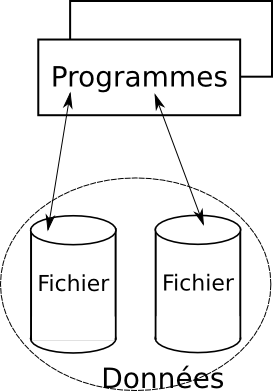
\includegraphics{images/ApprocheParApplication.png} & 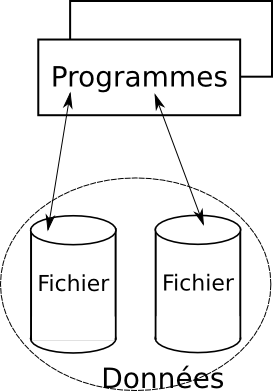
\includegraphics{images/ApprocheParApplication.png}
                \end{tabular}
            \end{center}
        \caption{Approche par application}
        \end{figure}

        Ces approches ont conduit à la « crise du logiciel ».

        \paragraph{Inconvénients}
            \begin{itemize}
                \item Redondance de données : les données sont dupliquées autant de fois qu'on en a besoin dans les différentes applications
                    \begin{itemize}
                        \item perte de place : déperdition de stockage
                        \item danger d'incohérence des données lors des mises à jour
                    \end{itemize}
                \item Dépendance entre données et programmes d'où maintenance accrue
                \item Dépendance entre niveaux logique et physique : vision de l'utilisateur des données et ce qui est effectivement stocké sur son disque
                \item Difficulté de développer de nouvelles applications non prévues (informatique décisionnelle)
            \end{itemize}

        \paragraph{Avantage} : démarche relativement facile à mettre en œuvre et progressive

    \section{Approche base de données}

        % Schéma de l'approche base de données
        \begin{figure}[H]
            \begin{center}
                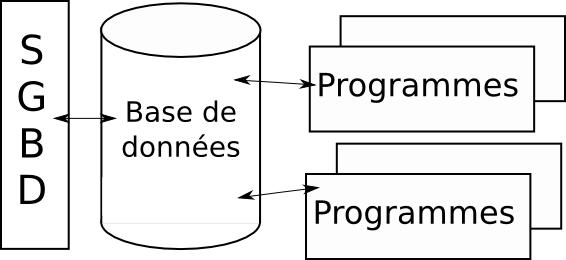
\includegraphics{images/ApprocheBaseDeDonnees.png}
            \end{center}
            \caption{Approche base de données}
        \end{figure}

        \textbf{SGBD} : Système de Gestion de Bases de Données

        \paragraph{Avantages}
            \begin{itemize}
                \item Élimination de la redondance de données
                \item Indépendance données/programmes
                \item Indépendance entre niveaux logique et physique
                \item Facilité de développer de nouvelles applications non prévues
            \end{itemize}

        \paragraph{Inconvénients} démarche longue, coûteuse, difficile à mettre en œuvre

        \paragraph{Modèles de bases de données}
            \begin{itemize}
                \item Modèle hiérarchique (1960)
                \item Modèle Codasyl (1964)
                \item Modèle relationnel (1970)
                \item Modèle orienté objet (1990)
            \end{itemize}

\newpage
\part{Le modèle relationnel}
    \section{Introduction}
        \subsection{3 composantes}
            \subsubsection*{Les concepts relationnels}
                Domaine, relations, tuples, attributs, clef primaire, clef étrangère, relation statique, relation dynamique, schéma relationnel.

            \subsubsection*{Algèbre relationnel}
                Projection, sélection, jointure, division, union, intersection, différence.

            \subsubsection*{Contraintes d'intégrité relationnelle}
                Intégrité de domaine, inéligibilité de relation, intégrité de références.

        \subsection{Rappels mathématiques}
            \subsubsection*{Produit cartésien}
                Soient $A$ et $B$ deux ensembles tels que :
                $$A\times B = \left\{(a,b)/a\in A, b\in B\right\}$$

                Exemple :
                $$A=\left\{1,2,3\right\} \: B=\left\{4,5\right\}$$
                $$A\times B = \left\{(1,4),(1,5),(2,4),(2,5),(3,4),(3,5)\right\}$$

            \subsubsection*{Relation binaire}
                Soient $A$ et $B$ deux ensembles et $R\subseteq A\times B$ une relation entre les éléments de $A$ et de $B$. $R$ contient les couples de $A\times B$.

                Exemple :
                $$R_1=\left\{a_1,b_1\right\} \: R_2=\left\{(a_1,b_1),(a_2,b_2)\right\}$$

    \section{Concepts relationnels}
        \subsection{Domaine sémantique}
            Un domaine sémantique est un ensemble de valeurs atomiques, ou simples. Chaque domaine est caractérisé par un type de base (numérique : entier, réel; alphanumérique : string, date,...).

            \paragraph{Exemple}
                \begin{itemize}
                    \item D\_NOMAV = Domaine de nom des avions
                    \item D\_NOMPIL = Domaine de nom des pilotes
                    \\
                    \item D\_NOMAV = \{'A310','A330','A340','B727','B747'\}
                    \item D\_NOMPIL = \{'DUPONT','ROGER'\}
                \end{itemize}

            Le domaine sémantique a comme objectif de vérifier la validité des comparaisons (évite de comparer D\_NOMPIL avec D\_NOMAV).

        \subsection{Relations/tuples}
            Soient $D_1,D_2,...,D_n$, $n$ domaines non nécessairement distincts. Une relation $R$ est le sous-ensemble du produit cartésien de ces $n$ domaines :
            $$R\subseteq D_1\times D_2 \times \dots \times D_n$$

            La relation en base de données est une relation $n$-aire avec des $n$-uplets comme éléments.

            \paragraph{Exemple}
                \begin{itemize}
                    \item AVION
                        \begin{itemize}
                            \item D\_NUMAV
                            \item D\_NOMAV
                            \item D\_CAP
                            \item D\_VILLE
                        \end{itemize}
                    \item AVION$\subseteq$D\_NUMAV$\times$D\_NOMAV$\times$D\_CAP$\times$D\_VILLE
                \end{itemize}

            \paragraph{Tuple} représente un avion : (100,'A310',250','MARSEILLE')

            \subsubsection{Représentation tabulaire d'une relation}
                AVION=\{(100,'A310',250,'MARSEILLE'),(200','B747',450,'PARIS')\}\\

                % Représentation tabulaire de la relation AVION
                \begin{table}[H]
                    \begin{center}
                        \begin{tabular}{|l|l|l|l|l|}
                            \hline
                            AVION & NUMAV & NOMAV & CAP & VILLE \\
                            \hline
                            \multirow{2}*{ } & 100   & A310  & 250 & MARSEILLE \\
                            \cline{2-5}      & 200   & B747  & 450 & PARIS \\
                            \hline
                        \end{tabular}
                    \end{center}
                    \caption{Représentation tabulaire de la relation AVION}
                \end{table}

                Ici,
                \begin{itemize}
                    \item AVION est l'en-tête
                    \item NUMAV, NOMAV, CAP, VILLE sont les attributs
                    \item Le corps est constitué des différents tuples
                    \item Les tuples sont les différentes lignes du tableau
                    \item Le corps est l'extension du schéma relationnel
                    \item L'en-tête est le schéma de la relation/intention
                \end{itemize}

        \subsection{Attributs}
            L'attribut est un rôle joué par un domaine dans une relation pour éliminer les ambiguïtés (D\_VILLE$\times$D\_VILLE).

            VOL$\subseteq$D\_NUMVOL$\times$D\_VILLE$\times$D\_VILLE$\times$D\_HEURE$\times$D\_HEURE\\
            Attribut NUMVOL, VILLE\_DEP, VILLE\_ARR, H\_DEP, H\_ARR

            Un attribut joue un rôle dans un domaine, un domaine a un type défini.

            Ainsi, (IT100, 'PARIS', 'LONDRES', 18, 20) avec les attributs
            \begin{itemize}
                \item D\_NUMVOL $\Rightarrow$ NUMVOL
                \item D\_VILLE $\Rightarrow$ VILLE\_DEP
                \item D\_VILLE $\Rightarrow$ VILLE\_ARR
                \item D\_HEURE $\Rightarrow$ HEURE\_DEP
                \item D\_HEURE $\Rightarrow$ HEURE\_ARR
            \end{itemize}
            Chaque attribut est défini sur un domaine.

        \subsection{Clef primaire}
            Une clef primaire est un attribut, ou groupe d'attributs, permettant d'identifier de manière unique les tuples de la relation.

            \paragraph{Exemple}  NUMAV ne contient aucun doublon, et est ainsi le domaine de clef primaire de la relation AVION.

        \subsection{Domaine primaire}
            C'est le domaine dans lequel est défini un attribut, une clef primaire.

            \paragraph{Exemple}
                \begin{itemize}
                    \item D\_NUMAV : domaine primaire
                    \item NUMAV : clef primaire
                \end{itemize}

        \subsection{Clef étrangère}
            C'est un attribut, ou groupe d'attribut, défini sur un ou plusieurs domaines primaires, qui est clef primaire dans une autre relation.

            \paragraph{Exemple}
                \begin{itemize}
                    \item AVION(\underline{NUMAV}, NOMAV, CAP, LOC)
                    \item VOL(\underline{NUMVOL}, NUMAV\#, NUMPIL\#, VILLE\_DEP, VILLE\_ARR, HEURE\_DEP, HEURE\_ARR)
                    \item PILOTE(\underline{NUMPIL}, NOMPIL, ADR, SALAIRE)
                \end{itemize}

        \subsection{Schéma relationnel}
            C'est le schéma de chaque relation, la liste des attributs. La clef étrangère sert à exprimer des liens sémantiques entre les relations du schéma relationnel. C'est l'ensemble du schéma de relations liées à travers des clefs primaires et étrangères. Chaque schéma de relation est décrit par le nom de la relation et la liste de ses attributs : AVION(NUMAV, NOMAV, CAP, LOC).

        \subsection{Autres concepts}
            \subsubsection*{Degré et cardinalité d'une relation}
                Le degré d'une relation est le nombre d'attributs d'une relation.

                La cardinalité d'une relation est le nombre de ses tuples.

            \subsubsection*{Relations dynamiques et statiques}
                Une relation dynamique est une relation qui contient une clef étrangère.

                Une relation statique est une relation indépendante, qui ne contient pas de clef étrangère.

            \subsubsection*{Attributs comparables ou compatibles}
                Deux attributs sont comparables ou compatibles s'ils sont définis sur le même domaine.

    \section{Contraintes d'intégrité relationnelles}
        \subsection{Contraintes d'intégrité statique/structurelle}
            Ce sont les règles de cohérence de la base induite par les concepts relationnels. Elles sont invariantes et ne dépendant pas de l'application.

            \subsubsection*{Contrainte de domaine}
                Toute valeur affectée à un attribut doit être dans le domaine de l'attribut.

            \subsubsection*{Contrainte de relation}
                Toute valeur affectée à la clef primaire doit être unique et obligatoire (doit exister).

            \subsubsection*{Contrainte de référence}
                Toute valeur affectée à la clef étrangère doit exister dans la clef primaire associée.

        \subsection{Contraintes dynamiques/applicatives}
            Les règles de cohérence de la base de données dépendent de l'application.

            \paragraph{Exemple}
                Pour un vol, on a VILLE\_DEP$<>$VILLE\_ARR et HEURE\_DEP$<>$HEURE\_ARR.
                
            La contrainte statique est vérifiée automatiquement par le SGBD. Les contraintes dynamiques sont spécifiées et programmées par l'administrateur de la base de données.

    \section{Algèbre relationnel}
        \subsection{Généralités}
            \subsubsection*{Opérateurs relationnels}
                \paragraph{Relation unaire}
                    Projection, séléction.

                \paragraph{Relation binaire}
                    Jointure, division.

            \subsubsection*{Opérateurs ensemblistes}
                \begin{itemize}
                    \item Union, qui s'apparente à un OR
                    \item Intersection, qui s'apparente à un AND
                    \item Différence, qui s'apparente à un NOT
                \end{itemize}

        \subsection{Opérateurs relationnels}
            \subsubsection{Projection}
                \paragraph{Définition}
                    Soit $R(U)$ une relation d'attributs U telle que
                    \begin{itemize}
                    	\item $U=\left\{A_1, A_2, \dots, A_n\right\}, X\subseteq U$
						\item $RS=\mathrm{PROJECTION}(R/X)$
						\item $RS=\left\{t(X)/r\subset R\right\}$
                    \end{itemize}

				\newpage
                \paragraph{Exemple : quels sont les noms et adresses des pilotes ?}

                    % Représentation tabulaire de la relation PILOTE
                    \begin{table}[H]
                        \begin{center}
                            \begin{tabular}{|l|l|l|l|l|}
                                \hline
                                PILOTE & NUMPIL & NOMPIL & ADR & SALAIRE \\
                                \hline
                                \multirow{3}*{ } & 100   & Dupont & Marseille & 5000 \\
                                \cline{2-5}      & 200   & Durand & Marseille & 4000 \\
                                \cline{2-5}      & 300   & Martin & Nice      & 3000 \\
                                \hline
                            \end{tabular}
                        \end{center}
                        \caption{Représentation tabulaire de la relation PILOTE}
                    \end{table}

                    \subparagraph{$RS=\mathrm{PROJECTION}(PILOTE/NOMPIL,ADR)$}
                        ~\\ % Ligne vide pour bien placer la figure
                        \begin{table}[H]
                            \begin{center}
                                \begin{tabular}{|l|l|l|}
                                    \hline
                                    RS  & NOMPIL    & ADR   \\
                                    \hline
                                    \multirow{3}*{ }      & Dupont  & Marseille \\
                                    \cline{2-3}           & Durand  & Marseille \\
                                    \cline{2-3}           & Martin  & Nice \\
                                    \hline
                                \end{tabular}
                            \end{center}
                            \caption{Projection de PILOTE sur NOMPIL et ADR}
                        \end{table}

                    \subparagraph{$RS=\mathrm{PROJECTION}(PILOTE/ADR)$}
                        ~\\ % Ligne vide pour bien placer la figure
                        \begin{table}[H]
                            \begin{center}
                                \begin{tabular}{|l|l|}
                                    \hline
                                    RS  & ADR   \\
                                    \hline
                                    \multirow{2}*{ }      & Marseille   \\
                                    \cline{2-2}           & Nice        \\
                                    \hline
                                \end{tabular}
                            \end{center}
                            \caption{Projection de PILOTE sur ADR}
                        \end{table}

                        La projection élimine les doublons.

                \paragraph{Propriétés}
                    \begin{itemize}
                        \item $\mathrm{Degr\acute{e}}(RS)\le\mathrm{Degr\acute{e}}(R)$
                        \item $\mathrm{Cardinalit\acute{e}}(RS)\le\mathrm{Cardinalit\acute{e}}(R)$
                    \end{itemize}

            \subsubsection{Sélection}
                Soient $R(U)$ une relation d'attributs $U=\left\{A_1,A_2,\dots,A_n\right\}$ constante et $Ai$ une valeur dans le domaine de $A$.

                $$RS=\mathrm{SELECTION}(R/Ai\theta \mathrm{constante})$$

                $\theta$ est l'un des opérateurs suivants : $=$, $<$, $>$, $<>$\footnote{opérateur de différence, équivalent à $!=$}, $\le$, $\ge$.

                \paragraph{Exemple : chercher les pilotes habitant à Marseille}~\\
                $RS=\mathrm{SELECTION}(PILOTE/ADR='\mathrm{MARSEILLE}')$
                    \begin{table}[H]
                        \begin{center}
                            \begin{tabular}{|l|l|l|l|l|}
                                \hline
                                RS & NUMPIL & NOMPIL & ADR & SALAIRE    \\
                                \hline
                                \multirow{2}*{ }      & 100 & Dupond & Marseille & 5000 \\
                                \cline{2-5}           & 200 & Durand & Marseille & 4000 \\
                                \hline
                            \end{tabular}
                        \end{center}
                        \caption{Pilotes habitant à Marseille}
                    \end{table}

                    \subparagraph{Propriétés}
                        \begin{itemize}
                            \item $\mathrm{Degr\acute{e}}(RS)=\mathrm{Degr\acute{e}}(R)$
                            \item $\mathrm{Cardinalit\acute{e}}(RS)\le\mathrm{Cardinalit\acute{e}}(R)$
                        \end{itemize}

                        On a ainsi les opérateurs suivants :
                        \begin{itemize}
                            \item La projection : sert à découper verticalement une relation
                            \item La sélection : sert à découper horizontalement une relation
                        \end{itemize}

                        \emph{Toujours commencer par la sélection}

                \paragraph{Exemple : quels sont les noms des pilotes habitant à Marseille ?}
                    \begin{itemize}
                        \renewcommand{\labelitemi}{ } % Pas de puce
                        \item $R1=\mathrm{SELECTION}(PILOTE/ADR='Marseille')$
                        \item $RS=\mathrm{PROJECTION}(R1/NOMPIL)$
                    \end{itemize}

                    \begin{table}[H]
                        \begin{center}
                            \begin{tabular}{|l|l|}
                                \hline
                                RS & NOMPIL \\
                                \hline
                                \multirow{2}*{ } & Dupont \\
                                \cline{2-2} & Durand \\
                                \hline
                            \end{tabular}
                        \end{center}
                        \caption{Sélection et projection}
                    \end{table}

            \subsubsection{Jointure}
                La jointure est un opérateur binaire : elle nécessite deux relations.

                Soient $R(U_1), S(U_2)$ deux relations d'attributs $U_1=\left\{A_1,A_2,\dots,A_n\right\}$ et $U_2=\left\{B_1,B_2,\dots,B_n\right\}$ et $A_i\in U_1, B_j\in U_2$ deux attributs compatibles.

                $$RS=\mathrm{JOINTURE}(R,S/A_i\theta B_j)$$
                $$RS=\left\{(t,s)/t\in R, s\in S,t(A_i)\theta S(B_j)\right\}$$
                avec $\theta$ un opérateur de comparaison.

                Le schéma de $RS$ contient tous les attributs de $A$ et tous les attributs de $S$.
                \begin{table}[H]
                    \begin{center}
                        \begin{tabular}{|l|l|l|l|}
                            \hline
                            R & A & B & C \\
                            \hline
                            \multirow{3}*{ } & $a_1$ & $b_1$ & $c_1$ \\
                            \cline{2-4}      & $a_2$ & $b_1$ & $c_1$ \\
                            \cline{2-4}      & $a_3$ & $b_2$ & $c_1$ \\
                            \hline
                        \end{tabular}
                        \quad
                        \begin{tabular}{|l|l|l|}
                            \hline
                            S & A & D \\
                            \hline
                            \multirow{4}*{ } & $a_1$ & $d_1$ \\
                            \cline{2-3}      & $a_1$ & $d_2$ \\
                            \cline{2-3}      & $a_2$ & $d_3$ \\
                            \cline{2-3}      & $a_2$ & $d_4$ \\
                            \hline
                        \end{tabular}
                        \quad
                        \begin{tabular}{|l|l|l|l|l|l|}
                            \hline
                            RS & A & B & C & A & D \\
                            \hline
                            \multirow{4}*{ } & $a_1$ & $b_1$ & $c_1$ & $a_1$ & $d_1$ \\
                            \cline{2-6}      & $a_1$ & $b_1$ & $c_1$ & $a_1$ & $d_2$ \\
                            \cline{2-6}      & $a_2$ & $b_1$ & $c_1$ & $a_2$ & $d_3$ \\
                            \cline{2-6}      & $a_2$ & $b_1$ & $c_1$ & $a_2$ & $d_4$ \\
                            \hline
                        \end{tabular}
                    \end{center}
                    \caption{Jointure entre $R$ et $S$ sur $A$}
                \end{table}

                \paragraph{Exemple : quels sont les noms des pilotes en service ?}
                    ~\\ % Ligne vide pour bien placer la figure
                    \begin{table}[H]
                        \begin{center}
                            \begin{tabular}{|l|l|l|l|l|}
                                \hline
                                PILOTE & NUMPIL & NOMPIL & ADR & SAL \\
                                \hline
                                \multirow{3}*{ } & 10 & Dupont & Nice & 5000 \\
                                \cline{2-5}      & 20 & Durand & Marseille & 6000 \\
                                \cline{2-5}      & 30 & Dupont & Marseille & 4000 \\
                                \hline
                            \end{tabular}
                            \vskip15pt
                            \begin{tabular}{|l|l|l|l|l|l|}
                                \hline
                                VOL & NUMVOL & NUMPIL & NUMAV & VILLE\_DEP & VILLE\_ARR \\
                                \hline
                                \multirow{3}*{ } & IT100 & 10 & 100 & Marseille & Paris \\
                                \cline{2-6}      & IT200 & 10 & 100 & Paris     & Marseille \\
                                \cline{2-6}      & IT300 & 30 & 200 & Toulous   & Paris \\
                                \hline
                            \end{tabular}
                        \end{center}
                        \caption{Relations PILOTE et VOL}
                    \end{table}

                    \begin{itemize}
                        \renewcommand{\labelitemi}{ } % Pas de puce
                        \item $R1=\mathrm{JOINTURE}(PILOTE,VOL/NUMPIL=NUMPIL)$
                        \item $RS=\mathrm{PROJECTION}(R1/NOMPIL)$
                    \end{itemize}

                    \begin{table}[H]
                        \begin{center}
                            \begin{tabular}{|l|l|l|l|l|l|l|l|l|l|}
                                \hline
                                R1 & NUMPIL & NOMPIL & ADR & SAL & NUMVOL & NUMPIL & NUMAV & VILLE\_DEP & VILLE\_ARR \\
                                \hline
                                \multirow{3}*{ } & 10 & Dupont & Nice & 5000 & IT100 & 10 & 100 & Marseille & Paris \\
                                \cline{2-10} & 10 & Dupont & Nice & 5000 & IT200 & 10 & 100 & Paris & Marseille \\
                                \cline{2-10} & 30 & Dupont & Marseille & 4000 & IT300 & 30 & 200 & Toulouse & Paris \\
                                \hline
                            \end{tabular}
                            \vskip15pt
                            \begin{tabular}{|l|l|}
                                \hline
                                RS & NOMPIL \\
                                \hline
                                \multirow{2}*{ } & Dupont \\
                                \cline {2-2} & Dupont \\
                                \hline
                            \end{tabular}
                        \end{center}
                        \caption{Jointure entre PILOTE et VOL sur NUMPIL}
                    \end{table}

                \paragraph{Différents types de jointures}
                    \subparagraph{Équijointure}
                    $$RS=\mathrm{JOINTURE}(PILOTE,VOL/NUMPIL=NUMPIL)$$

                    \subparagraph{Jointure naturelle}~\\
                        Enlève la deuxième occurreence d'un attribut identique (ici, enlève NUMPIL).

                        \begin{table}[H]
                            \begin{center}
                                \begin{tabular}{|l|l|l|l|l|l|l|l|l|}
                                    \hline
                                    RS & NUMPIL & NOMPIL & ADR & SAL & NUMVOL & NUMAV & VILLE\_DEP & VILLE\_ARR \\
                                    \hline
                                    \multirow{3}*{ } & 10 & Dupont & Nice & 5000 & IT100 & 100 & Marseille & Paris \\
                                    \cline{2-9} & 10 & Dupont & Nice & 5000 & IT200 & 100 & Paris & Marseille \\
                                    \cline{2-9} & 30 & Dupont & Marseille & 4000 & IT300 & 200 & Toulouse & Paris \\
                                    \hline
                                \end{tabular}
                            \end{center}
                            \caption{Jointure naturelle entre PILOTE et VOL sur NUMPIL}
                        \end{table}

                    \subparagraph{Jointure par $<>$}
                        $$RS=\mathrm{JOINTURE}(PILOTE,VOL/NUMPIL<>NUMPIL)$$

                         \begin{table}[H]
                            \begin{center}
                                \begin{tabular}{|l|l|l|l|l|l|l|l|l|l|}
                                    \hline
                                    RS & NUMPIL & NOMPIL & ADR & SAL & NUMVOL & NUMPIL & NUMAV & VILLE\_DEP & VILLE\_ARR \\
                                    \hline
                                    \multirow{6}*{ } & 10 & Dupont & Nice & 5000 & IT300 & 30 & 200 & Toulouse & Paris \\
                                    \cline{2-10}     & 20 & Durand & Marseille & 6000 & IT100 & 10 & 100 & Marseille & Paris \\
                                    \cline{2-10}     & 20 & Durand & Marseille & 6000 & IT200 & 10 & 100 & Paris & Marseille \\
                                    \cline{2-10}     & 20 & Durand & Marseille & 6000 & IT300 & 30 & 200 & Toulouse & Paris \\
                                    \cline{2-10}     & 30 & Dupont & Marseille & 4000 & IT100 & 10 & 100 & Marseille & Paris \\
                                    \cline{2-10}     & 30 & Dupont & Marseille & 4000 & IT200 & 10 & 100 & Paris & Marseille \\
                                    \hline
                                \end{tabular}
                            \end{center}
                            \caption{Jointure entre PILOTE et VOL avec NUMPIL$<>$NUMPIL}
                        \end{table}

                    \subparagraph{Autojointure}
                        $$RS=\mathrm{JOINTURE}(PILOTE,PILOTE/NUMPIL=NUMPIL)$$
                        \begin{table}[H]
                            \begin{center}
                                \begin{tabular}{|l|l|l|l|l|l|l|l|l|}
                                    \hline
                                    RS & NUMPIL & NOMPIL & ADR & SAL & NUMPIL & NOMPIL & ADR & SAL \\
                                    \hline
                                    \multirow{3}*{ } & 10 & Dupont & Nice & 5000 & 10 & Dupont & Nice & 5000 \\
                                    \cline{2-9}      & 20 & Durand & Marseille & 6000 & 20 & Durand & Marseille & 6000 \\
                                    \cline{2-9}      & 30 & Dupont & Marseille & 4000 & 30 & Dupont & Marseille & 4000 \\
                                    \hline
                                \end{tabular}
                            \end{center}
                            \caption{Autojointure de PILOTE sur NUMPIL}
                        \end{table}
            \subsubsection{Division}
                Soient $R(B,A)$ et $S(A)$ deux relations respectivement binaire et unaire, avec $A_r$ et $A_s$ définis sur le même domaine.
                $$RS=\mathrm{DIVISION}(R,S/A_r,A_s)$$
                $A_r$ et $A_s$ n'ont pas forcément le même nom.
                $$RS=\left\{t(B)/t\in R,\forall s\in S,(t(B),S(A))\in R\right\}$$

                \paragraph{Contraintes} $R$ a deux attributs, $S$ un seul. Les attributs de la division doivent être compatibles.

                $$RS=\mathrm{DIVISION}(R,S/A,A)$$
                \begin{table}[H]
                    \begin{center}
                        \begin{tabular}{|l|l|l|}
                            \hline
                            R & B & A \\
                            \hline
                            \multirow{3}*{ } & $b_1$ & $a_1$ \\
                            \cline{2-3}      & $b_1$ & $a_2$ \\
                            \cline{2-3}      & $b_2$ & $a_1$ \\
                            \hline
                        \end{tabular}
                        \begin{tabular}{|l|l|}
                            \hline
                            S & A \\
                            \hline
                            \multirow{2}*{ } & $a_1$ \\
                            \cline{2-2}      & $a_2$ \\
                            \hline
                        \end{tabular}
                        \begin{tabular}{|l|l|}
                            \hline
                            RS & B \\
                            \hline
                            & $b_1$ \\
                            \hline
                        \end{tabular}
                    \end{center}
                    \caption{Division de R par S}
                \end{table}

                $b_1$ est associé dans $R$ à toutes les valeurs de $A$.
                $$B=\left\{b_1,b_2\right\}\Rightarrow\left\{(b_1,a_1),(b_1,a_2)\right\}$$
                Or $b_2$ n'est pas associé dans $R$ à $a_2$ donc il n'est pas conservé.

                \paragraph{Remarques}
                \begin{itemize}
                    \item \emph{La division exprime « tous les », ou bien « au moins tous les » $\Rightarrow\;\forall$}
                    \item \emph{La jointure exprime « un », « il existe » $\Rightarrow\;\exists$}
                \end{itemize}

                \paragraph{Exemple : numéros des pilotes qui conduisent tous les avions de sa compagnie}
                ~\\
                NUMAV est l'attribut de la division.

                \begin{itemize}
                    \renewcommand{\labelitemi}{ } % Pas de puce
                    \item $R1=\mathrm{PROJECTION}(AVION/NUMAV)$
                    \item $R2=\mathrm{PROJECTION}(VOL/NUMAV,NUMPIL)$
                    \item $RS=\mathrm{DIVISION}(R1,R2/NUMAV,NUMAV)$
                \end{itemize}

                Les pilotes apparaissant dans le résultant sont associés à tous les avions de la compagnie.

		\newpage
        \subsection{Opérateurs ensemblistes}
            ~\\ % Ligne vide pour bien placer la figure
            \begin{figure}[H]
                \begin{center}
                    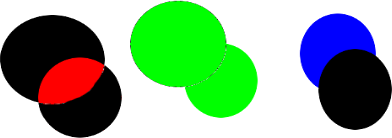
\includegraphics[scale=0.5]{images/OperateursEnsemblistes.png}
                \end{center}
                \caption{Opérateurs ensemblistes}
            \end{figure}

            \begin{itemize}
                \item \textcolor{red}{ROUGE : } intersection ($R\cap S$; $RS=\mathrm{INTERSECTION}(R,S)=\left\{t/t\in R\land t\in S\right\}$)
                \item \textcolor{green}{VERT : } union ($R\cup S$; $RS=\mathrm{UNION}(R,S)=\left\{t/t\in R\lor t\in S\right\}$)
                \item \textcolor{blue}{BLEU : } différence ($R-S$; $RS=\mathrm{DIFFERENCE}(R,S)=\left\{t/t\in R\land t\notin S\right\}$)
            \end{itemize}

            $R$ et $S$ sont uni-compatibles si :
            \begin{itemize}
                \item $\mathrm{Degr\acute{e}}(R)=\mathrm{Degr\acute{e}}(S)$
                \item Les attributs de $R$ et $S$ sont définis sur le même domaine
            \end{itemize}

            \paragraph{Exemple}~\\
                Soient $R(A,B,C)$ et $S(D,E,F)$ des relations. $R$ et $S$ sont uni-compatibles si
                \begin{itemize}
                    \item $A$ est sur le même domaine que $D$
                    \item $B$ est sur le même domaine que $E$
                    \item $C$ est sur le même domaine que $F$
                \end{itemize}

            \paragraph{Exemple : noms des pilotes habitant Nice et gagnant 5000\euro}
                \begin{itemize}
                    \renewcommand{\labelitemi}{ } % Pas de puce
                    \item $R1=\mathrm{SELECTION}(PILOTE/ADR='Nice')$
                    \item $R2=\mathrm{SELECTION}(PILOTE/SAL=5000)$
                    \item $R3=\mathrm{INTERSECTION}(R1,R2)$
                    \item $RS=\mathrm{PROJECTION}(R3/NOMPIL)$
                \end{itemize}
                \vskip15pt
                \begin{itemize}
                    \renewcommand{\labelitemi}{ } % Pas de puce
                    \item $R1=\mathrm{SELECTION}(PILOTE/ADR='Nice')$
                    \item $R2=\mathrm{SELECTION}(R1/SALAIRE=5000)$
                    \item $RS=\mathrm{PROJECTION}(R2/NOMPIL)$
                \end{itemize}

            \paragraph{Exemple : noms des pilotes qui n'ont jamais assuré de vol}
                \begin{itemize}
                    \renewcommand{\labelitemi}{ } % Pas de puce
                    \item $R1=\mathrm{PROJECTION}(VOL/NUMPIL)$
                    \item $R2=\mathrm{PROJECTION}(PILOTE/NUMPIL)$
                    \item $R3=\mathrm{DIFFERENCE}(R2,R1)$
                    \item $R4=\mathrm{JOINTURE}(PILOTE,R3/NUMPIL=NUMPIL)$
                    \item $RS=\mathrm{PROJECTION}(R4/NOMPIL)$
                \end{itemize}

\newpage
\part{Dépendances fonctionnelles}
    \section{Définition}
        Soient $r(R)$ une relation d'attributs $R$ et $x,y\in R$. $y$ dépend fonctionnellement de $x$, ou $x$ détermine $y$, ou $x$ implique $y$, $X\rightarrow Y$, si et seulement si $\forall t,t'\in r$. Si $t(x)=t'(x)$, alors $t(y)=t'(y)$, tous les tuples ayant même valeur sur $x$ ont même valeur sur $y$, à chaque valeur de $x$ correspond au plus une valeur de $y$, $\underbrace{|r(x,y)|}_{\text{Cardinalité de }r(x,y)}=\underbrace{|r(x)[}_{\text{Cardinalité de }r(x)}$.

    \section{Axiomes d'Armstrong}
        \subsection{Réflexivité}
            Si $y\subseteq X$ alors $x\rightarrow y$ ($x\rightarrow x$).

        \subsection{Augmentation}
            Si $x\rightarrow y$ et $w\subseteq z$ alors $x,z\rightarrow y,w$ ($x,z\rightarrow y$ si $w=\emptyset$).

        \subsection{Transitivité}
            Si $x\rightarrow y$ et $y\rightarrow z$ alors $x\rightarrow z$.

        \subsection{Pseudo-transitivité}
            Si $x\rightarrow y$ et $y,z \rightarrow t$ alors $x,y\rightarrow t$.

        \subsection{Décomposition}
            Si $x\rightarrow y,z$ alors $x\rightarrow y$ et $x\rightarrow z$.

        \subsection{Union}
            Si $x\rightarrow y$ et $x\rightarrow z$ alors $x\rightarrow y,z$.

    \section{Dépendance fonctionnelle minimale}
        $X\rightarrow A$ est une dépendance fonctionnelle minimale si et seulement si
        \begin{itemize}
            \item $A$ est un attribut unique (les cibles de la DF\footnote{dépendance fonctionnelle} minimale comportent un seul attribut)
            \item $\forall x\in X, X-x\nrightarrow A$ (tous les attributs de la source de la DF sont nécessaires)
        \end{itemize}

        \paragraph{Exemple}
            \begin{itemize}
                \item $D\rightarrow A$ est une DF minimale (car $\emptyset\nrightarrow A$)
                \item $BD\rightarrow A$ n'est pas une DF minimale (car $D\rightarrow A$, $B$ n'est pas nécessaire)
            \end{itemize}    

    \section{Clef candidate}
        $X\subseteq \mathbb{R}$ est une clef candidate si et seulement si $X\rightarrow \mathbb{R}$.

    \section{Clef candidate minimale}
        $X\subseteq \mathbb{R}$ est une clef candidate minimale si et seulement si
        \begin{itemize}
            \item $X$ est une clef candidate minimale
            \item $\forall x\in X, X-x\nrightarrow \mathbb{R}$ (tous les attributs de $X$ sont nécessaires pour déterminer $R$)
        \end{itemize}

    \section{Clef primaire}
        $X\subseteq \mathbb{R}$ est une clef primaire si et seulement si $X$ est une clef candidate minimale.

        \paragraph{Critères de choix d'une clef primaire parmi les clefs candidates minimales}
            \begin{enumerate}
                \item nombre d'attributs (choisir le plus petit)
                \item type (les types numériques sont prioritaires)
            \end{enumerate}

    \section{Attributs non-clef}
        $A\in \mathbb{R}$ est un attribut non-clef si et seulement si $A$ n'est pas une clef candidate minimale.

\newpage
\part{Théorie de modélisation}
    \section{Objectif}
        Un bon schéma relationnel est un schéma relationnel qui présente le moins de redondance de données et le moins d'anomalies de stockage dans un environnement de mise à jour.

        \subsection{Mauvais schéma relationnel}
            \begin{table}[H]
                \begin{center}
                    \begin{tabular}{|l|l|l|l|}
                        \hline
                        ENSEIGNANT       & NOM      & FONCTION  & SALAIRE   \\
                        \hline
                        \multirow{6}*{ } & CICCHETI & PROF      & 5000      \\
                        \cline{2-4}      & MIRANDA  & PROF      & 5000      \\
                        \cline{2-4}      & LAKHAL   & PROF      & 5000      \\
                        \cline{2-4}      & DUPONT   & ASSISTANT & 2000      \\
                        \cline{2-4}      & CASALI   & MC        & 4000      \\
                        \cline{2-4}      & LAPORTE  & MC        & 4000      \\
                        \hline
                    \end{tabular}
                \end{center}
                \caption{Mauvais schéma relationnel}
            \end{table}

            Ce schéma relationnel est mauvais :
            \begin{itemize}
                \item \textbf{Redondance de données} : (Prof,5000) se répète plusieurs fois
                \item \textbf{Anomalie de stockage} lors des opérations de mises à jour
                    \begin{itemize}
                        \item Ajout d'une nouvelle fonction et d'un nouveau salaire (exemple : (-,MA,3000)) impossible car la valeur de la clef primaire n'est pas définie
                        \item Baisser le salaire des professeurs nécessite plusieurs opérations
                        \item Supprimer l'enseignant DUPONT fait perdre de l'information (les assistants gagnent 2000\euro).
                    \end{itemize}
            \end{itemize}

        \subsection{Bon schéma relationnel}
            \begin{table}[H]
                \begin{center}
                    \begin{tabular}{|l|l|l|}
                        \hline
                        ENSEIGNANT       & NOM      & FONCTION  \\
                        \hline
                        \multirow{4}* {} & CICCHETI & PROF      \\
                        \cline{2-3}      & MIRANDA  & PROF      \\
                        \cline{2-3}      & DUPONT   & MA        \\
                        \cline{2-3}      & CASALi   & MC        \\
                        \hline
                    \end{tabular}
                    \quad
                    \begin{tabular}{|l|l|l|}
                        \hline
                        FONCTION         & FONCTION & SALAIRE   \\
                        \hline
                        \multirow{3}* {} & PROF     & 5000      \\
                        \cline{2-3}      & MA       & 3000      \\
                        \cline{2-3}      & MC       & 4000      \\
                        \hline
                    \end{tabular}
                \end{center}
                \caption{Bon schéma relationnel}
            \end{table}

    \section{Formes normales}
        Il y a trois formes normales : 1NF, 2NF et 3NF. Plus le degré de normalité d'une relation est important, moins on a de redondances de données et d'anomalie de stockage dans un contexte de mise à jour.

        \subsection{1NF (1\up{st} Normal Form)}
            Une relation $r(\mathbb{R})$ est en 1NF si et seulement si tous les attributs de $r(\mathbb{R})$ sont mono-valués (pour tout tuple de $r$, chaque attribut prend une seule valeur).

            \paragraph{Exemple de relation N1NF}
                ~\\ % Ligne vide pour bien placer la figure
                \begin{table}[H]
                    \begin{center}
                        \begin{tabular}{|l|l|l|l|}
                            \hline
                            LIVRE            & CODE     & TITRE     & AUTEUR    \\
                            \hline
                            \multirow{3}*{}  & $C_1$    & $T_1$     & $A_1$     \\
                            \cline{2-4}      & $C_2$    & $T_2$     & $A_1,A_2$ \\
                            \cline{2-4}      & $C_3$    & $T_4$     & $A_2,A_3,A_4$ \\
                            \hline
                        \end{tabular}
                    \end{center}
                    \caption{Relation N1NF}
                \end{table}

                AUTEUR est un attribut multivalué, LIVRE n'est donc pas en 1NF.

            \subsubsection{Normalisation en 1NF}
                \paragraph{Cas 1 : ajout d'attributs}
                ~\\ % Ligne vide pour bien placer la figure
                \begin{table}[H]
                    \begin{center}
                        \begin{tabular}{|l|l|l|l|l|l|}
                            \hline
                            LIVRE            & CODE     & TITRE     & AUTEUR 1  & AUTEUR 2  & AUTEUR 3  \\
                            \hline
                            \multirow{3}*{}  & $C_1$    & $T_1$     & $A_1$     &           &           \\
                            \cline{2-6}      & $C_2$    & $T_2$     & $A_1$     & $A_2$     &           \\
                            \cline{2-6}      & $C_3$    & $T_4$     & $A_2$     & $A_3$     & $A_4$     \\
                            \hline
                        \end{tabular}
                    \end{center}
                    \caption{Ajout d'attributs}
                \end{table}

                \paragraph{Cas 2 : ajout d'une relation toute clef}
                ~\\ % Ligne vide pour bien placer la figure
                \begin{table}[H]
                    \begin{center}
                        \begin{tabular}{|l|l|l|}
                            \hline
                            LIVRE            & CODE     & TITRE \\
                            \hline
                            \multirow{3}*{}  & $C_1$    & $T_1$ \\
                            \cline{2-3}      & $C_2$    & $T_2$ \\
                            \cline{2-3}      & $C_3$    & $T_4$ \\
                            \hline
                        \end{tabular}
                        \begin{tabular}{|l|l|l|}
                            \hline
                            AUTEURS          & \underline{CODE} & \underline{AUTEUR} \\
                            \hline
                            \multirow{6}*{}  & $C_1$            & $A_1$              \\
                            \cline{2-3}      & $C_2$            & $A_1$              \\
                            \cline{2-3}      & $C_2$            & $A_2$              \\
                            \cline{2-3}      & $C_3$            & $A_2$              \\
                            \cline{2-3}      & $C_3$            & $A_3$              \\
                            \cline{2-3}      & $C_3$            & $A_3$              \\
                            \hline
                        \end{tabular}
                    \end{center}
                    \caption{Relation toute clef}
                \end{table}

        \subsection{2NF (2\up{nd} Normal Form)}
            Une relation $r(\mathbb{R})$ est en 2NF si et seulement si :
            \begin{itemize}
                \item elle est en 1NF
                \item il n'y a pas de DF entre une partie d'une clef candidate minimale et un attribut qui n'appartient pas à une clef candidate minimale
            \end{itemize}

            \paragraph{DF problématique} $\underbrace{X}_{\text{une partie d'une CCM}} \rightarrow \underbrace{A}_{\text{un attribut qui n'appartient pas à une CCM}}$

            \paragraph{Exemple} COMMANDE(NO\_PROD, NO\_FOURN, NOM\_FOURN, QTE\_FOURN) avec
            $$\mathbb{F}_{\text{commande}} = \left\{\begin{array}{l}
                \text{NO\_PROD, NO\_FOURN} \rightarrow \text{NOM\_FOURN, QTE\_FOURN} \\
                \underbrace{\text{NO\_PROD}}_{\text{une partie d'une CCM}} \rightarrow \underbrace{\text{NOM\_FOURN}}_{\notin\text{ CCM}}
            \end{array}\right.$$
            Une seule clef candidate minimale : (NO\_PROD,NO\_FOURN).\\
            COMMANDE n'est pas en 2NF.

            \subsubsection{Normalisation en 2NF}
                Théorème de décomposition de Casey-Delabel :\\
                « Soit $r(\mathbb{R})$ une relation, avec $x,y\subseteq\mathbb{R}$ et $x\rightarrow y$. On a $r=\mathrm{JointureNaturelle}(r_1,r_2/x=x)$ avec $r_1=\mathrm{Projection}(r/x,y)$ et $r_2=\mathrm{Projection}(r/y,x)$. »

                Ce théorème nous garantit que la décomposition de $r(x,y,z)$ en $r_1(x,y)$ et $r_2(x,z)$ est réversible (sans perte d'information).

                \paragraph{Exemple de normalisation en 2NF}~\\
                COMMANDE(NO\_PROD, NO\_FOURN, NOM\_FOURN, QTE\_FOURN) devient :\\
                COMMANDE(\underline{NO\_PROD,NO\_FOURN},QTE\_FOURN)\\
                $\underbrace{r_1}_{\text{FOURNISSEUR}}(\underline{\text{NO\_FOURN}},\text{NOM\_FOURN})$\\

                \paragraph{Remarque} lorsque les clefs candidates minimales ne comportent qu'un seul attribut, la relation est automatiquement en 2NF.

        \subsection{3NF (3\up{rd} Normal Form)}
            Une relation $r(\mathbb{R})$ est en 3NF si et seulement si :
            \begin{itemize}
                \item $r(\mathbb{R})$ est en 2NF
                \item il n'y a pas de DF entre un attribut ou groupe d'attributs qui n'est pas une clef candidate minimale, et un attribut qui n'appartient pas à une clef candidate minimale
            \end{itemize}

            \paragraph{DF problématique} $\underbrace{X}_{\text{n'est pas une CCM}} \rightarrow \underbrace{A}_{\notin\text{ CCM}}$

            \subsubsection{Normalisation en 3NF}
            PRODUIT(\underline{NO\_PROD}, LIBELLE, CODE\_TVA, TAUX\_TVA) avec
            $$\mathbb{F}_{\text{PRODUIT}} = \left\{\begin{array}{l}
                \text{NO\_PROD} \rightarrow \text{LIBELLE, CODE\_TVA, TAUX\_TVA}\\
                \text{CODE\_TVA} \rightarrow \text{TAUX\_TVA}
            \end{array}\right.$$
            devient :\\
            TVA(\underline{CODE\_TVA}, TAUX\_TVA)\\
            PRODUIT(\underline{NO\_PROD}, LIBELLE, CODE\_TVA)

\newpage
\part{Algorithmes et méthodes de normalisation}
    Objectif : aider à la conception d'un schéma relationnel en 3NF

    \section{Concepts de base}
        \subsection{Dérivabilité des DF}
            Soit $\mathbb{F}$ un ensemble de DF sur $r(\mathbb{R})$ et $x,y\subseteq\mathbb{R}$. On dit que $x\rightarrow y$ est dérivable à partir de $\mathbb{F}(\mathbb{F}\vdash x\rightarrow y)$ si $x\rightarrow y$ peut être obtenue à partir de $\mathbb{F}$ en appliquant les axiomes d'Armstrong.

            \paragraph{Exemple}
            $$\mathbb{F}=\left\{\begin{array}{l}
                A\rightarrow B\\
                B\rightarrow C\\
            \end{array}\right.$$
			
		\subsection{Couverture d'un ensemble de DF}
			Soit $\mathbb{F}$ un ensemble de DF sur $r(\mathbb{R})$. $\mathbb{G}$ est une couverture de $\mathbb{F}$ si et seulement si :
			\begin{itemize}
				\item $\mathbb{F}\vdash\mathbb{G}$ ($\forall x \rightarrow A\in\mathbb{G},\mathbb{F}\vdash x\rightarrow A$)
				\item $\mathbb{G}\vdash\mathbb{F}$ ($\forall x \rightarrow A\in\mathbb{F},\mathbb{G}\vdash x\rightarrow A$)
			\end{itemize}

			$\mathbb{G}$ est une couverture de $\mathbb{F}$ et $\mathbb{F}$ est une couverture de $\mathbb{G}$.
			
		\subsection{Couverture minimale d'un ensemble de DF}
			Soit $\mathbb{F}$ un ensemble de DF. $\mathbb{M}$ est une couverture minimale de $\mathbb{F}$ si et seulement si :
			\begin{itemize}
				\item Toutes les DF de $\mathbb{M}$ sont de la forme $X\Rightarrow A$ (un attribut cible)
				\item $\forall x\rightarrow A\in\mathbb{M},\forall x\in X,\mathbb{M}\forall X-x\rightarrow A$ (chaque DF de $\mathbb{M}$ est minimale)
				\item $\forall x\rightarrow A\in\mathbb{M},\mathbb{M}-\left\{x\rightarrow A\right\}\vdash X\rightarrow A$ (chaque DF de $\mathbb{M}$ est nécessaire)
			\end{itemize}

			Si ces trois conditions sont vraies alors $\mathbb{M}$ est une couverture minimale de $\mathbb{F}$.
			
		\subsection{Fermeture d'Armstrong}
			Soit $\mathbb{F}$ un ensemble de DF sur $r(\mathbb{R})$ et $Z_1,Z_2,\hdots,Z_n$ une suite cumulative ($Z_1\subseteq Z_2\subseteq Z_3\hdots\subseteq Z_n$). La fermeture d'Armstrong d'un ensemble d'attributs selon un ensemble de DF est notée $(X^+_\mathbb{F})$.
			
			\subsubsection{Application +}
				$S(\mathbb{R})\rightarrow P(\mathbb{R})$
				
				$X\rightarrow X^+_\mathbb{F}=Z_n$ avec $Z_{n+1}=Z_n, Z_1=X, Z_n=Z_{n-1}\cup\left\{A\in\mathbb{R}/x\rightarrow A\in\mathbb{F},X\subseteq Z_{n-1}\right\}$
				
			\subsubsection{Exemple : $BD^+_\mathbb{F}$, la fermeture de $BD$ selon $\mathbb{F}$}
				$$BD^+_\mathbb{F}=Z_n$$
				$$Z_1=BD$$
				$$Z_2=BD\cup\left\{E,A\right\}=ABDE$$
				$$Z_3=ABDE\cup\left\{C\right\}=ABCDE$$
				$$Z_4=ABCDE\cup\left\{\mathbb{F}\right\}=Z_3$$
				$X^+_\mathbb{F}=X\cup\text{tous les attributs déterminés par X (directement ou indirectement)}$
			
	\section{Algorithmes de normalisation}
		\subsection{Algorithme de calcul d'une clef candidate minimale}
			\begin{itemize}
				\item Entrée : $\mathbb{F}$ un ensemble de DF sur $r(\mathbb{R})$
				\item Sortie : $X\subseteq\mathbb{R}$ une clef candidate minimale pour $r(\mathbb{R})$
			\end{itemize}
			
			\paragraph{Algorithme}
			\begin{tabbing}
				$X:=\mathbb{R}$\\
				Pour \= tout $A\in\mathbb{R}$\\
				\> si $(X-A)^+_\mathbb{F}=\mathbb{R}$ alors $X:=X-A$\\
				Renvoyer $X$
			\end{tabbing}
			
		\subsection{Algorithme de calcul d'une couverture minimale}
			\paragraph{Étapes de calcul}
				\begin{enumerate}
					\item Décomposer les DF (un seul attribut cible par DF)
					\item Suppression des attributs de la source de chaque DF
					\item Suppression des DF redondantes
				\end{enumerate}
				
		\subsection{Algorithme de calcul de la fermeture d'Armstrong}
			\begin{itemize}
				\item Entrée : $\mathbb{F}$ un ensemble de DF sur $r(\mathbb{R})$ et $X\leq\mathbb{R}$
				\item Sortie : $X^+_\mathbb{F}$ la fermeture de $X$ selon $\mathbb{F}$
			\end{itemize}
			
			\paragraph{Algorithme}
			\begin{tabbing}
				Fermeture$:=X$\\
				Répé\=ter\\
				\>DF$:=X$\\
				\>Pour \= tout $X\rightarrow A\in\mathbb{F}$ faire\\
				\>\>Si $x\leq$Fermeture et $A\notin$Fermeture alors Fermeture$:=$Fermeture$\cup A$\\
				Jusqu'à DF$=$Fermeture\\
				Renvvoyer Fermeture
			\end{tabbing}
			
\newpage
\part{Modélisation de bases de données}
	Jusqu'à présent, nous avons présenté des approches de conception faisant abstraction de l'univers réel. À partir d'une liste d'attributs et d'un ensemble de dépendances fonctionnelles, on arrivait à trouver le schéma normalisé relationnel directement. Cette approche a des limites :
	\begin{itemize}
		\item l'identification des DF est ardue voire impossible du premier coup
		\item les algorithmes ont un coût qui augmente exponentiellement avec le nombre d'attributs
		\item un schéma relationnel est difficilement compréhensible pour l'utilisateur/client
	\end{itemize}
	
	Pour résoudre ces problèmes, on va ajouter une phase à la conception de la base de données :\\
	\begin{figure}[H]
		\begin{center}
			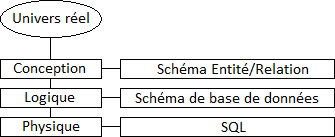
\includegraphics{images/ConceptionBD.png}
		\end{center}
		\caption{Conception de base de données}
	\end{figure}
	
	\section{Schéma entité/relation}
		\paragraph{Définition} Le schéma entité/relation est une représentation statique. Il a pour but de décrire simplement les données ainsi que les liens pouvant exister.
			
		\subsection{Les types d'entités}
			Une entité est la représentation d'un objet (matériel ou immatériel) identifiable de l'univers réel. Par exemple, une voiture dont le numéro de série est X123. Comme en programmation orientée objet, où les objets similaires sont regroupés en classe, les entités sont regroupées en types d'entités.
			
			Un type d'entité est la description d'entités qui possèdent les mêmes caractéristiques. Par abus de langage, il peut arriver d'utiliser le mot « entité » à la place de « type d'entité ». Pour parler d'entités, préférer « occurrence ». Pour parler de type d'entité, préférer « TE ».
			
			\begin{figure}[H]
				\begin{center}
					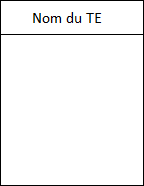
\includegraphics{images/RepresentationTE.png}
				\end{center}
				\caption{Représentation graphique d'un type d'entité}
			\end{figure}
			
		\subsection{Les propriétés}
			Une propriété (ou attribut) est une information élémentaire (c'est à dire non déductible d'autres informations) qui présent un intérêt pour le domaine étudié. L'ensemble de valeurs permises pour une propriété est son domaine.
			
			Il faut être vigilant en choisissant le nom d'une propriété car il ne doit pas être ambigu.

			\begin{figure}[H]
				\begin{center}
					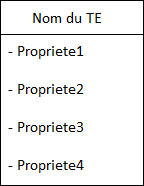
\includegraphics{images/RepresentationProprietes.png}
				\end{center}
				\caption{Représentation graphique des proprietés}
			\end{figure}
			
		\subsection{Les identifiants (ou clefs)}
			L'identifiant d'un TE est un ensemble de propriétés dont la valeur permet d'identifier de manière unique une entité (occurrence).
			
			\begin{figure}[H]
				\begin{center}
					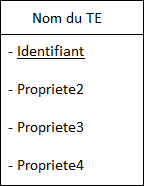
\includegraphics{images/RepresentationIdentifiants.png}
				\end{center}
				\caption{Représentation graphique des identifiants}
			\end{figure}
			
		\subsection{Associations et types d'associations}
			Une association (ou relation) est un lien sémantique entre plusieurs entités (occurrences).
			
			Un type d'association est un ensemble d'associations qui partagent les mêmes caractéristiques.
			
			\begin{figure}[H]
				\begin{center}
					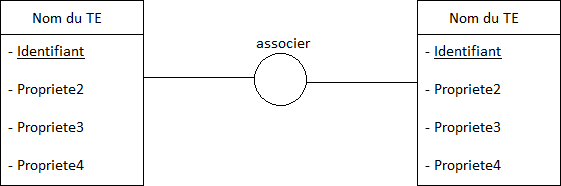
\includegraphics{images/RepresentationAssociation.png}
				\end{center}
				\caption{Représentation graphique d'une association}
			\end{figure}
			
			\subsubsection{Associations}
			~\\
				\begin{figure}[H]
					\begin{center}
						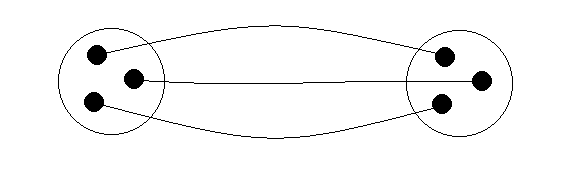
\includegraphics{images/AssociationUnAUn.png}
					\end{center}
					\caption{Association « un-à-un »}
				\end{figure}
				
				\begin{figure}[H]
					\begin{center}
						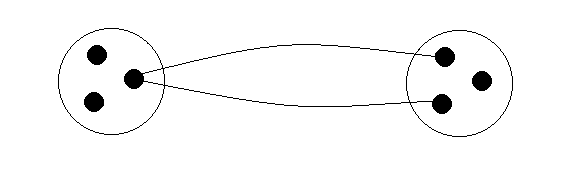
\includegraphics{images/AssociationUnAPlusieurs.png}
					\end{center}
					\caption{Association « un-à-plusieurs »}
				\end{figure}
				
				\begin{figure}[H]
					\begin{center}
						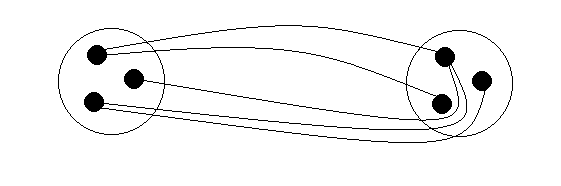
\includegraphics{images/AssociationPlusieursAPlusieurs.png}
					\end{center}
					\caption{Association « plusieurs-à-plusieurs »}
				\end{figure}
				
			\subsubsection{Cardinalités}
				Les cardinalités permettent de caractériser la multiplicité du lien qui existe entre les occurrences et l'association à laquelle elle est reliée. La cardinalité d'un type d'association (TA) est le nombre de fois minimal et maximal qu'une entité peut intervenir dans une association de ce type.
				
				Une TA dont l'une des cardinalités est (n,1) est dite hiérarchique.
				
				\begin{figure}[H]
					\begin{center}
						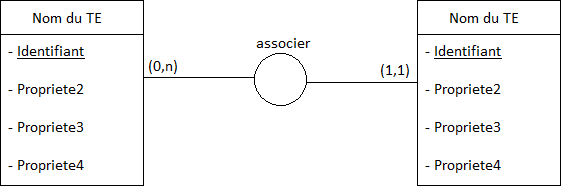
\includegraphics{images/RepresentationCardinalite.png}
					\end{center}
					\caption{Représentation des cardinalités}
				\end{figure}
			
			\subsubsection{Dimension d'une TA}
				La dimension d'un TA est le nombre de TE qui participent à l'association.
				
				\begin{figure}[H]
					\begin{center}
						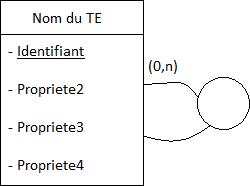
\includegraphics{images/TAUnaire.png}
					\end{center}
					\caption{TA unaire (reflective)}
				\end{figure}
				
				\begin{figure}[H]
					\begin{center}
						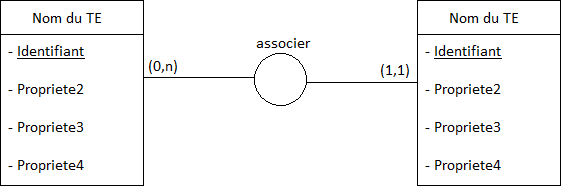
\includegraphics{images/TABinaire.png}
					\end{center}
					\caption{TA binaire}
				\end{figure}
				
				\begin{figure}[H]
					\begin{center}
						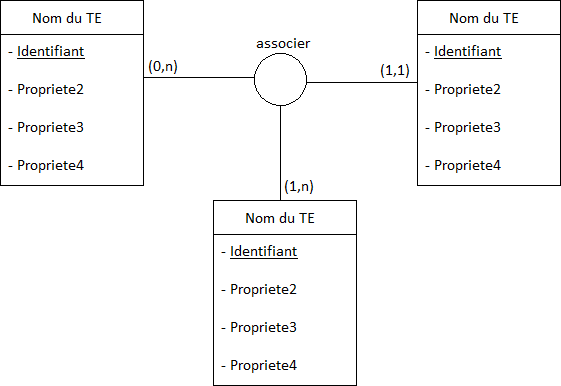
\includegraphics{images/TATernaire.png}
					\end{center}
					\caption{TA ternaire}
				\end{figure}
				
			\subsubsection{Identification d'une association}
				Une association n'a pas d'existence en dehors des entités liées. On utilise donc pour l'identifier la combinaison des clefs des TE liés. La valeur de l'identifiant doit être unique.
				
		\section{Dérivation relationnelle}
			La dérivation relationnelle est la transformation d'un schéma Entités/Associations en un schéma relationnel normalisé (3NF). Pour ce faire, on applique trois règles simples :
			\begin{enumerate}
				\item Dérivation des TE : 1 TE = 1 relation
				\item Dérivation des TA non-hiérarchiques : 1 TA non-hiérarchique = 1 relation. La clef primaire de la relation est l'identifiant du TA.
				\item Dérivation des TA hiérarchiques : 1 TA hiérarchique = 1 clef étrangère du côté de la cardinalité (n,1)
			\end{enumerate}
			
			%\paragraph{Exemple}
			~\\
			\begin{figure}[H]
				\begin{center}
					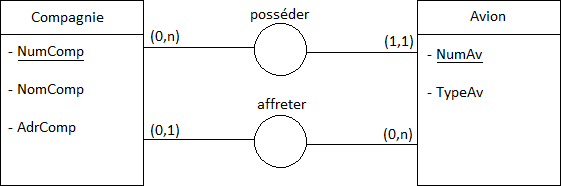
\includegraphics{images/DerivationRelationnelle.png}
				\end{center}
				\caption{Dérivation relationnelle}
			\end{figure}
			
			\begin{itemize}
				\item COMPAGNIE(\underline{NumComp}, NomComp, AdrComp)
				\item AVION(\underline{NumAv}, TypeAv, NumComp\#)
				\item AFFRETER(\underline{NumComp\#, NumAv\#})
			\end{itemize}
			
		\section{Règles de conception}
			\begin{enumerate}
				\item tout TE doit être identité (avoir une clef)
				\item tout TA non(hiérarchique doit être identifié par la combinaison des clefs des TE liés
				\item tout TE doit être normalisé (3NF)
				\item un TA hiérarchique ne doit pas avoir d'attribut
				\item un TA de degré supérieur à 1 ne peut pas être hiérarchique
			\end{enumerate}

\newpage
\part{Le langage SQL}
	SQL (Structured Query Language) prend trois aspects :
		\begin{itemize}
			\item langage de manipulation de données (LMD) : requêtes et mises à jours des données (\emph{\texttt{INSERT},\texttt{DELETE}, \texttt{UPDATE}})
			\item langage de définition de données (LDD) : manipulation de la structure, création de relations, ajout d'attributs,...
			\item langage de contrôle des données (LCD) : intégrité, confidentialité
		\end{itemize}
		
	SQL est une norme ANSI, mais suivant les SGBD, on a des variantes (dialectes) de SQL comme SQL*Plus d'Oracle.
	
	\section{SQL comme langage de manipulation des données (LMD)}
		Toute requêtes SQL s'exprime sous forme de blocs.
		
		\subsection{Expression des projections}\index{SELECT}
			Les attributs projetés sont mentionnés dans la clause \emph{\texttt{SELECT}}, séparés par des virgules.\index{FROM}
			\paragraph{Exemple : numéros et noms des pilotes}
				\begin{alltt}
					\begin{tabbing}
						\emph{SELECT} \= NumPil, NomPil\\
						\emph{FROM} \> PILOTE
					\end{tabbing}
				\end{alltt}
				
			Quand on doit conserver tous les attributs, on utilise \texttt{*}.
			
			En SQL, il n'y a pas d'élimination automatique des doublons. C'est à la charge de l'utilisateur grâce au mot-clef \emph{\texttt{DISTINCT}}.\index{DISTINCT}
			\paragraph{Exemple : numéros et noms des pilotes}
				\begin{alltt}
					\begin{tabbing}
						\emph{SELECT} \= \emph{DISTINCT} NumPil, NomPil\\
						\emph{FROM} \> PILOTE
					\end{tabbing}
				\end{alltt}
				
		\subsection{Expression des sélections}
			Les sélections s'expriment dans la clause \emph{\texttt{WHERE}} comme en langage algébrique.\index{WHERE}
			\paragraph{Exemple : numéros des pilotes habitant à Marseille}
				\begin{alltt}
					\begin{tabbing}
						\emph{SELECT} \= NumPil\\
						\emph{FROM} \> PILOTE\\
						\emph{WHERE} \> ADR='Marseille'
					\end{tabbing}
				\end{alltt}
				
			On peut combiner des conditions avec \emph{\texttt{AND}} et \emph{\texttt{OR}}.\index{AND}\index{OR}
			\paragraph{Exemple : numéros des pilotes nommés Dupont habitant à Marseille}
				\begin{alltt}
					\begin{tabbing}
						\emph{SELECT} \= NumPil\\
						\emph{FROM} \> PILOTE\\
						\emph{WHERE} \> \= ADR='Marseille'\\
									 \> \> \emph{AND} NOMPIL='Dupont'
					\end{tabbing}
				\end{alltt}
				
			\subsubsection{Prédicats de sélection}
				On peut utiliser les prédicats suivants dans la clause \emph{\texttt{WHERE}} :\index{BETWEEN}\index{IN}\index{LIKE}\index{IS NULL}
				\begin{itemize}
					\item \texttt{<attribut>} \emph{\texttt{BETWEEN}} \texttt{<valeur1>} \emph{\texttt{AND}} \texttt{<valeur2>}
					\item \texttt{<attribut>} \emph{\texttt{IN}}(\texttt{<valeur1>, <valeur2>,...})
					\item \texttt{<attribut>} \emph{\texttt{LIKE}} \texttt{'valeur\_générique\%'} (\_ = n'importe quel caractère, \% = n'importe quel nombre de caractères)
					\item \texttt{<attribut>} \emph{\texttt{IS NULL}}
				\end{itemize}
				
		\subsection{Calculs horizontaux}
			Ces calculs peuvent figurer soit dans la clause \emph{\texttt{SELECT}} (le résultat du calcul fait partie de la requête), soit dans la clause \emph{\texttt{WHERE}} (la condition porte sur le résultat du calcul).
			Il est possible d'utiliser les opérateurs +, -, *, / sur les nombres, + et - sur les dates, et || (concaténation) sur les chaines; il est aussi possible d'utiliser les fonctions \emph{\texttt{UPPER}} (passer une chaîne en majuscules), \emph{\texttt{LOWER}} (passer une chaîne en minuscule) et \emph{\texttt{LENGTH}} (renvoie la taille de la chaîne).\index{UPPER}\index{LOWER}\index{LENGTH}
			
		\subsection{Calculs verticaux}
			Les cinq fonctions classiques sont :
			\begin{itemize}
				\item \emph{\texttt{SUM}} (somme)\index{SUM}
				\item \emph{\texttt{AVG}} (moyenne)\index{AVG}
				\item \emph{\texttt{COUNT}} (comptage)\index{COUNT}
				\item \emph{\texttt{MIN}} (valeur minimum) \index{MIN}
				\item \emph{\texttt{MAX}} (valeur maximum) \index{MAX}
			\end{itemize}
			
			Un calcul vertical s'effectue une seule fois pour tous les tuples d'une relation. Il est possible de combiner les calculs horizontaux et verticaux.
			\paragraph{Exemple : donner le total des salaires des pilotes}
			\begin{alltt}
				\begin{tabbing}
					\emph{SELECT} \= \emph{SUM}(SAL)\\
					\emph{FROM} \> PILOTE
				\end{tabbing}
			\end{alltt}
			
			Les valeurs nulles sont ignorées. Le seul cas où \emph{\texttt{SUM}}, \emph{\texttt{AVG}}, \emph{\texttt{MIN}} et \emph{\texttt{MAX}} renvoient \emph{\texttt{NULL}} est quand toutes les valeurs sont nulles. Pour donner une valeur par défaut au lieu de \emph{\texttt{NULL}}, on utilise \emph{\texttt{NVL}}.\index{NVL}
			
			\paragraph{Exemple : somme des salaires et primes des pilotes}
			\begin{alltt}
				\begin{tabbing}
					\emph{SELECT} \= \emph{NVL}(\emph{SUM}(SAL),0) + \emph{NVL}(\emph{SUM}(Prime),0)\\
					\emph{FROM} \> PILOTE
				\end{tabbing}
			\end{alltt}
			
		\subsection{Jointures prédicatives}
			Elles s'expriment dans la clause \emph{\texttt{WHERE}} de la même façon qu'en langage algébrique : \texttt{<attribut1>} $\theta$ \emph{<attribut2>}, où $\theta$ est un opérateur de comparaison.
			
			\paragraph{Exemple : numéro des avions localisés dans la ville de départ du vol IT100}
				\begin{alltt}
					\begin{tabbing}
						\emph{SELECT} \= NUMAV\\
						\emph{FROM} \> AVION, VOL\\
						\emph{WHERE} \> NUMVOL='IT100' \emph{AND} LOC=VILLE_DEP
					\end{tabbing}
				\end{alltt}

			\paragraph{Exemple : numéro et nom des pilotes faisant au moins un vol au départ de Nice}
				\begin{alltt}
					\begin{tabbing}
						\emph{SELECT} \= \emph{DISTINCT} NOMPIL, PILOTE.NUMPIL\\
						\emph{FROM} \> PILOTE, VOL\\
						\emph{WHERE} \> VILLE_DEP='Nice' \emph{AND} PILOTE.NUMPIL=VOL.NUMPIL
					\end{tabbing}
				\end{alltt}
				
			\paragraph{Exemple : auto-jointure, nom des pilotes habitant la même ville que le pilote 100}
				\begin{alltt}
					\begin{tabbing}
						\emph{SELECT} \= P.NUMPIL\\
						\emph{FROM} \> PILOTE P, PILOTE P100\\
						\emph{WHERE} \> P100.NUMPIL=100 \emph{AND} P.VILLE=P100.VILLE
					\end{tabbing}
				\end{alltt}
				
		\subsection{Jointures imbriquées}
			Une jointure imbriquée s'exprime avec deux blocs : le premier bloc et un bloc imbriqué (ou sous-requête).
			
			\subsubsection{La sous-requête renvoie une seule valeur}
				\paragraph{Exemple : numéro des pilotes qui gagnent plus que la moyenne}
					\begin{alltt}
						\begin{tabbing}
							\emph{SELECT} \= NUMPIL\\
							\emph{FROM} \> PILOTE\\
							\emph{WHERE} \> SAL > (\= \emph{SELECT} \= \emph{AVG}(SAL) \=\\
												   \> \> \emph{FROM} \> PILOTE \>)
						\end{tabbing}
					\end{alltt}
					
					Le bloc imbriqué est exécuté en premier et une seule fois.
					
			\subsubsection{La sous-requête renvoie un seul tuple}
				\paragraph{Exemple : numéro des pilotes ayant la même adresse et le même salaire que le pilote 100}
					\begin{alltt}
						\begin{tabbing}
							\emph{SELECT} \= NUMPIL\\
							\emph{FROM} \> PILOTE\\
							\emph{WHERE} \> (ADR,SAL)=(\=\emph{SELECT} \= ADR,SAL\=\\
													\>\>\emph{FROM}   \> PILOTE\\
													\>\>\emph{WHERE}  \> NUMPIL=100)
						\end{tabbing}
					\end{alltt}
					
			\subsubsection{La sous-requête rend un ensemble de résultats}
				\paragraph{La comparaison se fait avec un des résultats du bloc imbriqué}
					\subparagraph{Exemple : numéro des vols faits par un Airbus} \index{ANY}
						\begin{alltt}
							\begin{tabbing}
								\emph{SELECT} \= NUMVOL\\
								\emph{FROM} \> VOL\\
								\emph{WHERE} \> NUMAV=\emph{ANY} (\=\emph{SELECT} \= NUMAV\\
																 \>\>\emph{FROM} \> AVION\\
																 \>\>\emph{WHERE} \> NUMAV \emph{LIKE} 'A%')
							\end{tabbing}
						\end{alltt}
						
					\subparagraph{Exemple : numéro des pilotes ayant le même salaire et la même adresse qu'un Dupont}
						\begin{alltt}
							\begin{tabbing}
								\emph{SELECT} \= NUMPIL\\
								\emph{FROM} \> PILOTE\\
								\emph{WHERE} \> (SAL,ADR)=\emph{ANY} (\=\emph{SELECT} \= SAL,ADR\\
																 \>\>\emph{FROM} \> PILOTE\\
																 \>\>\emph{WHERE} \> NUMPIL='Dupont')
							\end{tabbing}
						\end{alltt}
						
				\paragraph{La comparaison se fait avec tous les resultats du bloc imbriqué}
					\subparagraph{Exemple : numéro des pilotes marseillais gagnant plus que tous les pilotes parisiens}\index{ALL}
						\begin{alltt}
							\begin{tabbing}
								\emph{SELECT} \= NUMPIL\\
								\emph{FROM} \> PILOTE\\
								\emph{WHERE} \> ADR='Marseille' \emph{AND} SAL > \emph{ALL} (\=\emph{SELECT} \= SAL\\
																						\>\>\emph{FROM} \> PILOTE\\
																						\>\>\emph{WHERE} \> ADR='Paris')\\
							\end{tabbing}
						\end{alltt}
						
		\subsection{Opérateurs ensemblistes}
			Il faut que les clauses \emph{\texttt{SELECT}} des blocs comportent le même nombre d'attributs, et que ces attributs soient compatibles.
			
			\paragraph{Exemple : numéro des avions localisés à Paris ou faisant un vol au départ de Paris}\index{UNION}
				\begin{alltt}
					\begin{tabbing}
						\emph{SELECT} \= NUMAV\\
						\emph{FROM} \> AVION\\
						\emph{WHERE} \> LOC='Paris'\\
						\emph{UNION}\\
						\emph{SELECT} \> NUMAV\\
						\emph{FROM} \> VOL\\
						\emph{WHERE} \> VILLE_DEP='Paris'
					\end{tabbing}
				\end{alltt}
				
			\paragraph{Exemple : numéro des avions faisant un vol au départ de leur localisation}\index{INTERSECT}
				\begin{alltt}
					\begin{tabbing}
						\emph{SELECT} \= NUMAV, LOC\\
						\emph{FROM} \> AVION\\
						\emph{INTERSECT}\\
						\emph{SELECT} \> NUMAV, VILLE_DEP\\
						\emph{FROM} \> VOL\\
					\end{tabbing}
				\end{alltt}
				
			\paragraph{Exemple : numéro des avions n'effectuant aucun vol}\index{MINUS}
				\begin{alltt}
					\begin{tabbing}
						\emph{SELECT} \= NUMAV\\
						\emph{FROM} \> AVION\\
						\emph{MINUS}\\
						\emph{SELECT} \> NUMAV\\
						\emph{FROM} \> VOL\\
					\end{tabbing}
				\end{alltt}
				
			\paragraph{Remarque} avec les opérateurs ensemblistes, il y a élimination des doublons
			
		\subsection{Jointures externes}
			Une jointure classique entre $r_1$ et $r_2$ parcourt les tuples de $r_1$ et génère un résultat pour chaque tuple satisfaisant la condition de jointure. Une jointure externe procède de la même manière mais conserve les tuples de $r_1$ ne satisfaisant pas la condition de jointure.
			
			\paragraph{Exemple : jointure externe entre PILOTE et VOL avec NUMPIL=NUMPIL}
			~\\
			\begin{table}[H]
				\begin{center}
					\begin{tabular}{|r|c|}
						\hline
						PILOTE 	& NUMPIL \\
						\hline
								& 100 \\
								& 101 \\
								& 102 \\
								& 103 \\
						\hline
					\end{tabular}
					\begin{tabular}{|r|c|c|}
						\hline
						VOL	& NUMVOL	& NUMPIL \\
						\hline
							& IT100		& 100 \\
							& IT200		& 102 \\
							& IT300		& 100 \\
							& IT400		& 102 \\
						\hline
					\end{tabular}
					
					~\\
					\begin{tabular}{|r|c|c|c|}
						\hline
						JOINTURE	& NUMPIL	& NUMVOL	& NUMPIL \\
						\hline
									& 100		& IT100		& 100 \\
									& 100		& IT300		& 100 \\
									& 101		& \emph{\texttt{NULL}} & 101 \\
									& 102		& IT200		& 102 \\
									& 102		& IT400		& 102 \\
									& 103		& \emph{\texttt{NULL}} & 103 \\
						\hline
					\end{tabular}
				\end{center}
				\caption{Jointure externe}
			\end{table}
			
			En SQL, la jointure externe est indiquée par un \emph{\texttt{(+)}} derrière l'attribut de jointure qui pourra prendre des valeurs nulles :\index{(+)}
			\begin{alltt}
				\begin{tabbing}
					\emph{SELECT} \= *\\
					\emph{FROM}	\> PILOTE,VOL \\
					\emph{WHERE} \> PILOTE.NUMPIL=VOL.NUMPIL\emph{(+)}
				\end{tabbing}
			\end{alltt}
			
		\subsection{Test de non-existence de tuples}
			Pour ces requêtes, il faut vérifier qu'un tuple appartenant à un ensemble $E_1$ n'existe pas dans cet ensemble $E_2$. Par exemple, les pilotes ne faisant aucun vol. Il y a 5 formulations.
			
			\subsubsection{Jointure imbriquée avec \emph{\texttt{NOT IN}}}\index{IN}
				\begin{alltt}
					\begin{tabbing}
						\emph{SELECT} \= NUMPIL\\
						\emph{FROM} \> PILOTE\\
						\emph{WHERE} \> NUMPIL \emph{NOT IN} (\=\emph{SELECT} \= NUMPIL\=\\
															\>\>\emph{FROM} \> VOL\>)
					\end{tabbing}
				\end{alltt}
				
			\subsubsection{Jointure imbriquée avec \emph{\texttt{<> ALL}}}
				\begin{alltt}
					\begin{tabbing}
						\emph{SELECT} \= NUMPIL\\
						\emph{FROM} \> PILOTE\\
						\emph{WHERE} \> NUMPIL\emph{<>ALL} (\=\emph{SELECT} \= NUMPIL\=\\
															\>\>\emph{FROM} \> VOL\>)
					\end{tabbing}
				\end{alltt}
				
			\subsubsection{Différence ensembliste}
				\begin{alltt}
					\begin{tabbing}
						\emph{SELECT} \= NUMPIL\\
						\emph{FROM} \> PILOTE\\
						\emph{MINUS}\\
						\emph{SELECT} \= NUMPIL\\
						\emph{FROM} \> VOL\\
					\end{tabbing}
				\end{alltt}
				
			\subsubsection{Jointure externe et prédicat \emph{\texttt{IS NULL}}}
				\begin{alltt}
					\begin{tabbing}
						\emph{SELECT} \= *\\
						\emph{FROM}	\> PILOTE,VOL \\
						\emph{WHERE} \> PILOTE.NUMPIL=VOL.NUMPIL\emph{(+)}\\
									\> \emph{AND} NUMVOL \emph{IS NULL}
					\end{tabbing}
				\end{alltt}
				
			\subsubsection{Bloc imbriquée et prédicat \emph{\texttt{NOT EXISTS}}}\index{EXISTS}
				Devant un bloc imbriquée, \emph{\texttt{NOT EXISTS}} renvoie :
					\begin{itemize}
						\item vrai si le bloc imbriqué ne rend aucun résultat
						\item faux si le bloc imbriqué rend des résultats
					\end{itemize}
					
				\begin{alltt}
					\begin{tabbing}
						\emph{SELECT} \= NUMPIL\\
						\emph{FROM}	\> PILOTE\\
						\emph{WHERE} \> \emph{NOT EXISTS} (\=\emph{SELECT}\= *\\
														\>\>\emph{FROM}\> VOL)
					\end{tabbing}
				\end{alltt}
				
				Avec \emph{\texttt{NOT EXISTS}}, il faut une exécution corrélée des deux blocs : pour chaque tuple dans le premier bloc, il faut exécuter le bloc imbriqué. Pour cela, il faut exprimer une jointure entre les relations des deux blocs. Il faut donner un alias à la relation du premier bloc et faire la jointure avec cet alias dans le bloc imbriqué.
				
				\begin{alltt}
					\begin{tabbing}
						\emph{SELECT} \= NUMPIL\\
						\emph{FROM}	\> PILOTE P\\
						\emph{WHERE} \> \emph{NOT EXISTS} (\=\emph{SELECT}\= *\\
														\>\>\emph{FROM}\> VOL\\
														\>\>\emph{WHERE}\> VOL.NUMPIL=P.NUMPIL)
					\end{tabbing}
				\end{alltt}
				
		\subsection{Opérations de partitionnement}\index{GROUP BY}
			Partitionner une relation consiste à créer des classes d'équivalence (ou sous-ensembles) telles que :
			\begin{itemize}
				\item leur union soit égale à la relation de départ
				\item les classes d'équivalence soient disjointes deux à deux (pas de tuples en commun)
			\end{itemize}
			
			Le ou les critères permettant de créer ces classes sont les attributs de partitionnement. Par exemple, partitionner VOL sur NUMPIL consiste à créer trois classes d'équivalence (une par pilote). Chaque classe regroupe les vols d'un même pilote.
			
			Avec un partitionnement, on peut appliquer les fonctions agrégatives sur les classes d'équivalence.
			
			En SQL, le partitionnement se fait dans la clause \emph{\texttt{GROUP BY}} dans laquelle on indique le ou les attributs de partitionnement. Cette clause suit le \emph{\texttt{WHERE}}.
			
			\paragraph{Exemple : donner pour chaque pilote, le nombre de vols}
				\begin{alltt}
					\begin{tabbing}
						\emph{SELECT} \= NUMPIL, \emph{COUNT}(*)\\
						\emph{FROM} \> VOL\\
						\emph{GROUP BY} \> NUMPIL
					\end{tabbing}
				\end{alltt}
				
			\paragraph{Exemple : donner pour chaque pilote et chaque avion, le nombre de vols}
				\begin{alltt}
					\begin{tabbing}
						\emph{SELECT} \= NUMPIL, NUMAV, \emph{COUNT}(*)\\
						\emph{FROM} \> VOL\\
						\emph{GROUP BY} \> NUMPIL, NUMAV
					\end{tabbing}
				\end{alltt}
				
			\paragraph{Remarque} Avec un \emph{\texttt{GROUP BY}}, on peut combiner un attribut atomique avec une fonction agrégative à condition que ce soit l'attribut de partitionnement.
			
			\paragraph{Exemple : donner pour chaque pilote, le nombre de villes d'arrivées}
				\begin{alltt}
					\begin{tabbing}
						\emph{SELECT} \= NUMPIL, \emph{COUNT}(\emph{DISTINCT} VILLE_ARR)\\
						\emph{FROM} \> VOL\\
						\emph{GROUP BY} \> NUMPIL
					\end{tabbing}
				\end{alltt}
				
			\paragraph{Exemple : donner le salaire moyen et maximum des pilotes par ville de résidence, sauf Paris}
				\begin{alltt}
					\begin{tabbing}
						\emph{SELECT} \= ADR, \emph{AVG}(SAL), \emph{MAX}(SAL)\\
						\emph{FROM} \> PILOTE\\
						\emph{WHERE} \> ADR<>'Paris'\\
						\emph{GROUP BY} \> ADR
					\end{tabbing}
				\end{alltt}
				
			On peut exprimer des conditions sur des classes d'équivalence (conditions utilisant des fonctions agrégatives), on utilise la clause \emph{\texttt{HAVING}} qui suit le \emph{\texttt{GROUP BY}}.\index{HAVING}
			
			\paragraph{Exemple : donner pour chaque pilote faisant au moins 5 vols, le nombre de vols}
			\begin{alltt}
					\begin{tabbing}
						\emph{SELECT} \= NUMPIL\\
						\emph{FROM} \> PILOTE\\
						\emph{GROUP BY} \> NUMPIL\\
						\emph{HAVING} \> \emph{COUNT}(*)>=5
					\end{tabbing}
				\end{alltt}
				
			\paragraph{Exemple : donner le numero des pilotes faisant autant de vols que le pilote 100}
				\begin{alltt}
					\begin{tabbing}
						\emph{SELECT} \= NUMPIL\\
						\emph{FROM} \> PILOTE\\
						\emph{GROUP BY} \> NUMPIL\\
						\emph{HAVING} \> \emph{COUNT}(*)>=(\=\emph{SELECT} \= \emph{COUNT}(*)\\
															\>\>\emph{FROM} \> VOL\\
															\>\>\emph{WHERE} \> NUMPIL=100)
					\end{tabbing}
				\end{alltt}
				
			\paragraph{Remarque} \emph{\texttt{GROUP BY}} ne s'utilise pas avec \emph{\texttt{DISTINCT}}, et pas sur une clef primaire.
			
		\subsection{Recherche dans des arborescences}
			\subsubsection{Représentation des hiérarchies}
				\paragraph{Exemple : hiérarchie des lieux}
					~\\
					\begin{figure}[H]
						\begin{center}
							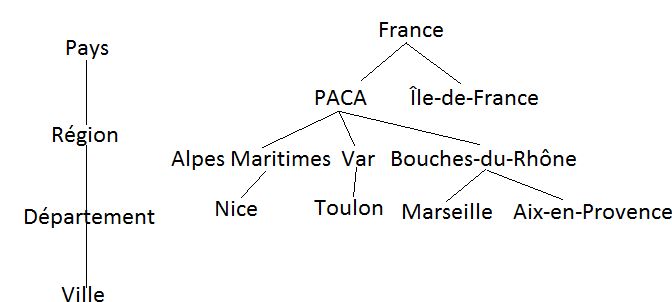
\includegraphics{images/HierarchieLieux.png}
						\end{center}
						\caption{Hiérarchie des lieux}
					\end{figure}

				\paragraph{Représentation avec le modèle entité/relation}
				~\\
					\begin{figure}[H]
						\begin{center}
							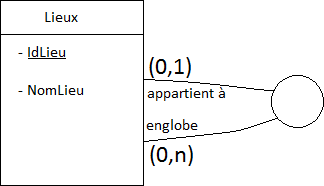
\includegraphics{images/HierarchieLieuxEA.png}
						\end{center}
						\caption{Hiérarchie des lieux avec le modèle entité/relation}
					\end{figure}
					
					\subparagraph{Remarque} Ce TA est hiérarchique.
					
				\paragraph{Représentation avec le modèle relationnel}
					\begin{itemize}
						\item Lieu(\underline{IdLieux}, Nom, IdLieuPere\#)
					\end{itemize}
					
			\subsubsection{Manipulation de hiérarchies}
				En SQL classique, il faut faire des auto-jointures.
				
				\paragraph{Exemple : liste des villes des Bouches-du-Rhône}
					\begin{alltt}
						\begin{tabbing}
							\emph{SELECT} \= LV.NomLieu\\
							\emph{FROM} \> LIEU LD, LIEU LV\\
							\emph{WHERE} \> \=LD.NomLieu='Bouches-du-Rhône'\\
										\>\>\emph{AND} LD.IdLIeu=LV.IdLieuPere
						\end{tabbing}
					\end{alltt}
					
				\paragraph{Exemple : liste des villes de PACA}
					\begin{alltt}
						\begin{tabbing}
							\emph{SELECT} \= LV.NomLieu\\
							\emph{FROM} \> LIEU LR, LIEU LD, LIEU LV\\
							\emph{WHERE} \> \=LR.NomLieu='PACA'\\
										\>\>\emph{AND} LR.IdLieu=LD.IdLieuPere\\
										\>\>\emph{AND} LD.IdLieu=LV.IdLieuPere\\
						\end{tabbing}
					\end{alltt}
					
				En SQL*Plus d'Oracle, la clause \emph{\texttt{CONNECT BY}} permet de parcourir des hiérarchies.\index{CONNECT BY}
				
				\begin{alltt}
					\begin{tabbing}
						\emph{SELECT} \=<liste_attributs>\\
						\emph{FROM} \><relation> -- Une seule relation\\
						[\emph{WHERE} \><liste_conditions>]\\
						\emph{CONNECT BY} \=[\emph{PRIOR}] <attribut_fils>=[\emph{PRIOR}] <attribut_pere>\\
									\>[\emph{AND} <condition_hierarchique>]\\
									\>[\emph{START WITH} <condition_depart>]\\
									\>[\emph{ORDER BY LEVEL}]
					\end{tabbing}
				\end{alltt}
				
				\begin{itemize}
					\item \emph{\texttt{CONNECT BY}} permet de donner le sens du parcours dans les hiérarchies. On met \emph{\texttt{PRIOR}} devant l'attribut fils pour une recherche descendante, ou devant l'attribut père pour une recherche ascendante. Par exemple, \emph{\texttt{CONNECT BY PRIOR}} \texttt{IdLieu=IdLieuPere} pour descendre dans la hiérarchie des lieux.
					
					\item \emph{\texttt{START WITH}} permet dedonner une condition de départ pour la recherche.
							\paragraph{Exemple : donner tous les lieux de la région PACA}
								\begin{alltt}
									\begin{tabbing}
										\emph{SELECT} \= NomLieu\\
										\emph{FROM} \>LIEU\\
										\emph{CONNECT BY} \= \emph{PRIOR} IdLieu=IdLieuPere\\
														\>\emph{START WITH} NomLieu='PACA'
									\end{tabbing}
								\end{alltt}
							
							\paragraph{Remarques}
								\begin{itemize}
									\item si plusieurs tuples satisfont la condition de départ, la recherche arborescente se fait pour chacun de ces tuples
									\item s'il n'y a pas de \emph{\texttt{START WITH}}, Oracle part de toutes les racines pour un parcours descendant, ou de toutes les feuilles pour un parcours ascendant
									\item on peut mettre des jointures imbriquées dans la clause \emph{\texttt{START WITH}}
								\end{itemize}
								
							\paragraph{Exemple : hiérarchie des localisations des villes de départ des vols}
								\begin{alltt}
									\begin{tabbing}
										\emph{SELECT} \= NomLieu\\
										\emph{FROM} \> LIEU\\
										\emph{CONNECT BY} \=IdLieu=\emph{PRIOR} IdLieuPere\\
														\>\emph{START WITH} NomLieu \emph{IN} (\=\emph{SELECT} \=Ville_Dep\=\\
																								\>\>\emph{FROM}\>VOL\>)
									\end{tabbing}
								\end{alltt}
								
					\item \emph{\texttt{AND}} permet d'éliminer de la recherche une partie de l'arbre. Si un nœud (tuple) ne satisfait pas cette condition, tous ses descendants sont éliminés (pour un parcours descendant), ou tous ses ascendants sont éliminés (pour un parcours ascendant).
						
						\paragraph{Exemple : hiérarchie des lieux, sauf ceux de la région PACA}
							\begin{alltt}
								\begin{tabbing}
									\emph{SELECT} \=NomLieu\\
									\emph{FROM} \>LIEU\\
									\emph{CONNECT BY} \=IdLieu=\emph{PRIOR} IdLieuPere\\
													\>\emph{AND} NomLieu<>'PACA'
								\end{tabbing}
							\end{alltt}
						\paragraph{Remarque} Si on met \texttt{NomLieu<>'PACA'} dans le \emph{\texttt{WHERE}}, la région PACA est éliminée du résultat mais pas ses départements ni ses villes.
						
						~\\
					\item \emph{\texttt{ORDER BY}} permet de trier les résultats.\index{ORDER BY}
						\paragraph{Exemple : liste alphabétique des pilotes}
							\begin{alltt}
								\begin{tabbing}
									\emph{SELECT} \=NOMPIL\\
									\emph{FROM}\>PILOTE\\
									\emph{ORDER BY} NOMPIL \emph{ASC}
								\end{tabbing}
							\end{alltt}
							
							On peut utiliser \emph{\texttt{DESC}} pour un tri inverse.
							~\\
							
					\item \emph{\texttt{LEVEL}} correspond au niveau. Le niveau 1 correspond aux premiers tuples sélectionnés.\index{LEVEL}
				\end{itemize}
				
		\subsection{Calculs imbriquées dans le \emph{\texttt{SELECT}} et le \emph{\texttt{FROM}}}
			\paragraph{Exemple : donner le numéro des pilotes, l'écart entre leur salaire et le salaire moyen}
			\subsubsection{Bloc imbriqué dans le \emph{\texttt{SELECT}}}
				Il faut que le bloc renvoie au plus un résultat.
				\begin{alltt}
					\begin{tabbing}
						\emph{SELECT}\= NUMPIL,SAL-(\=\emph{SELECT}\=\emph{AVG}(SAL)\=\\
												\>\>\emph{FROM} \>PILOTE\>)\\
						\emph{FROM}\> PILOTE
					\end{tabbing}
				\end{alltt}
				
			\subsubsection{Bloc imbriqué dans le \emph{\texttt{FROM}}}
				Le résultat est une relation temporaire. On peut donc l'imbriquer dans un \emph{\texttt{FROM}}.
				
				\begin{alltt}
					\begin{tabbing}
						\emph{SELECT}\= NUMPIL, SAL-SMOY\\
						\emph{FROM}\> PILOTE, (\=\emph{SELECT}\= \emph{AVG}(SAL) SMOY\=\\
												\>\>\emph{FROM} \>PILOTE\>)\\
					\end{tabbing}
				\end{alltt}
				
				\paragraph{Exemple : donner l'écart entre le salaire des pilotes et le salaire moyen de leur ville de résidence}
					\begin{alltt}
						\begin{tabbing}
							\emph{SELECT}\= NUMPIL, SAL-SMOY\\
							\emph{FROM}\> PILOTE, (\=\emph{SELECT}\= \emph{AVG}(SAL) SMOY,ADR\=\\
													\>\>\emph{FROM} \>PILOTE\\
													\>\>\emph{GROUP BY} ADR\>\>) PILSAL\\
							\emph{WHERE}\> PILOTE.ADR=PILSAL.ADR
						\end{tabbing}
					\end{alltt}
					
		\subsection{Expression des divisions}
			Il y a deux méthodes.
			
			\subsubsection{Avec \emph{\texttt{GROUP BY}} et comptage}
				\paragraph{Exemple : numéro des pilotes qui conduisent tous les avions (pilotes qui conduisent autant d'avions qu'il en existe)}
					\begin{alltt}
						\begin{tabbing}
							\emph{SELECT}\= NUMPIL\\
							\emph{FROM}\> VOL\\
							\emph{GROUP BY} NUMPIL\\
							\emph{HAVING} \> \emph{COUNT}(\emph{DISTINCT} NUMAV)=(\=\emph{SELECT}\= \emph{COUNT}(*)\=\\
																				\>\>\emph{FROM}\> AVION\>)
						\end{tabbing}
					\end{alltt}
					
				\paragraph{Exemple : numéro des pilotes qui conduisent tous les types d'appareils}
					\begin{alltt}
						\begin{tabbing}
							\emph{SELECT}\= NUMPIL\\
							\emph{FROM}\> VOL, AVION\\
							\emph{WHERE}\> VOL.NUMAV=AVION.NUMAV\\
							\emph{GROUP BY} NUMPIL\\
							\emph{HAVING} \> \emph{COUNT}(\emph{DISTINCT} NOMAV)=(\=\emph{SELECT}\= \emph{COUNT}(\emph{DISTINCT} NOMAV)\=\\
																				\>\>\emph{FROM}\> AVION\>)
						\end{tabbing}
					\end{alltt}
					
			\subsubsection{Avec un double \emph{\texttt{NOT EXISTS}}}
				\paragraph{Exemple : numéro des pilotes qui conduisent tous les avions (numéro des pilotes tels qu'il n'existe aucun avion qui ne soit pas conduit par ces pilotes)}
					\begin{alltt}
						\begin{tabbing}
							\emph{SELECT}\= NUMPIL\\
							\emph{FROM}\> PILOTE P\\
							\emph{WHERE} \> \emph{NOT EXISTS} (\=\emph{SELECT}\= *\\
															\>\>\emph{FROM}\> AVION A\\
															\>\>\emph{WHERE}\> \emph{NOT EXISTS} (\=\emph{SELECT}\= *\\
																							\>\>\>\>\emph{FROM}\> VOL\\
																							\>\>\>\>\emph{WHERE} \> VOL.NUMAV=A.NUMAV\\
																							\>\>\>\>			\> \emph{AND} VOL.NUMPIL=P.NUMPIL))
						\end{tabbing}
					\end{alltt}
				
				\newpage
				\paragraph{Exemple : numéro des pilotes qui conduisent au moins les mêmes avions que le pilote 100 (numéro des pilotes tels qu'il n'existe aucun avion non conduit par le pilote 100 qui ne soit pas conduit par eux)}
					\begin{alltt}
						\begin{tabbing}
							\emph{SELECT}\= NUMPIL\\
							\emph{FROM}\> PILOTE P\\
							\emph{WHERE} \> \emph{NOT EXISTS} (\=\emph{SELECT}\= *\\
															\>\>\emph{FROM}\> VOL V\\
															\>\>\emph{WHERE} \> NUMPIL=100\\
															\>\>\> \emph{AND NOT EXISTS} (\=\emph{SELECT}\= *\\
																							\>\>\>\>\emph{FROM}\> VOL\\
																							\>\>\>\>\emph{WHERE} \> P.NUMPIL=VOL.NUMPIL\\
																							\>\>\>\>			\> \emph{AND} V.NUMAV=VOL.NUMAV))
						\end{tabbing}
					\end{alltt}
		
	\section{SQL comme langage de contrôle des données (LCD)}
		\subsection{Concept de vue}\index{CREATE VIEW}
			UNe vue est une table virtuelle. On peut la voir comme une relation temporaire résultant d'une requête. On crée une vue ainsi : \emph{\texttt{CREATE VIEW}} \texttt{<nomvue>} \emph{\texttt{AS}} \texttt{<requete>}.
			
			\paragraph{Exemple : vue des pilotes habitant à Marseille}
				\begin{alltt}
					\begin{tabbing}
						\emph{CREATE VIEW} PIL_MARSEILLE \emph{AS}\\
						\emph{SELECT}\= NUMPIL, NOMPIL\\
						\emph{FROM} \> PILOTE\\
						\emph{WHERE} \> ADR='Marseille'
					\end{tabbing}
				\end{alltt}
				
		\subsection{Premier rôle des vues : limiter la consultation des données}
			Les vues permettent de limiter l'accès aux données à certains utilisateurs. L'utilisateur aura accès à une vue, mais ne pourra pas voir les attributs et tuples qui ne sont pas dans la vue. L'utilisateur peut manipuler les vues comme des relations.
			
		\subsection{Deuxième rôle des vues : écrire des requêtes complexes}
			\begin{alltt}
				\begin{tabbing}
					\emph{CREATE VIEW} VOL_HORAIRE \emph{AS}\\
					\emph{SELECT}\= NUMPIL, \emph{SUM}(HEURE_ARR-HEURE_DEP)\\
					\emph{FROM}\> VOL\\
					\emph{GROUP BY} NUMPIL
				\end{tabbing}
			\end{alltt}
			
			Pour mettre à jour une vue, il ne faut pas mettre de \emph{\texttt{GROUP BY}}, \emph{\texttt{CONNECT BY}}, \emph{\texttt{DISTINCT}}, fonctions agrégatives, opérateurs ensemblistes, dans le premier bloc.

\newpage
\appendix
\part{Mémento des ordres SQL*Plus}
	\section{SQL comme langage de définition de données (LDD)}
		Types syntaxiques des attributs : \texttt{VARCHAR2(n) CHAR[(n)] NUMBER[(n[,m)]] DATE LONG}
		
		\subsection{Création de relation}
			\begin{alltt}
				\begin{tabbing}
					\emph{CREATE TABLE} \= <nom_table>\\
					\> (<nom_colonne1> <type1> [\emph{DEFAULT} <expression1>]\\
					\>[, <nom_colonne2> <type2> [\emph{DEFAULT} <expression2>]]\\
					\>[, <contrainte1>[, <contrainte2>]])
				\end{tabbing}
				où :
				\begin{tabbing}
					<contraintei> = \emph{CONSTRAINT} <nom_contrainte> <spec_contrainte> [<etat>]\\
					<spec_contrainte> = \= \emph{PRIMARY KEY}(<attribut1[, <attribut2>, ...])\\
										\> | \= \emph{FOREIGN KEY}(<attribut1>[, <attribut2>,...]) \\
										\> \> \emph{REFERENCES} <nom_relation_associée>(<attribut1>[, <attribut2>,...]) \\
										\> \> [\emph{ON DELETE <CASCADE|SET NULL>}]\\
										\> | \emph{CHECK}(<nom_attribut | expression> <condition>)\\
					<etat> = \emph{ENABLE} | \emph{DISABLE}
				\end{tabbing}
				\emph{CREATE TABLE} <nom_relation> [(liste_attributs>, <liste_contraintes>)]
				\emph{AS} <requete>
			\end{alltt}
			
		\subsection{Ajout d'attributs et de contraintes dans une relation}
			\begin{alltt}
				\begin{tabbing}
					\emph{ALTER TABLE} <nom_table>\\
					\emph{ADD} (\=[nom_colonne1> <type1>] [\emph{DEFAULT} <expression1>] [\emph{NOT NULL}] [\emph{UNIQUE}]\\
								\>[,<nom_colonne2> <type2> [\emph{DEFAULT} <expression2>] [\emph{NOT NULL}] [\emph{UNIQUE}]...]\\
								\>[,<contrainte1> ...])
				\end{tabbing}
				où
				\begin{tabbing}
					<contraintei> = \emph{CONSTRAINT} <nom_contrainte> <spec_contrainte> [<etat>]\\
					<spec_contrainte> = \= \emph{PRIMARY KEY}(<attribut1[, <attribut2>, ...])\\
										\> | \= \emph{FOREIGN KEY}(<attribut1>[, <attribut2>,...]) \\
										\> \> \emph{REFERENCES} <nom_relation_associée>(<attribut1>[, <attribut2>,...]) \\
										\> \> [\emph{ON DELETE <CASCADE|SET NULL>}]\\
										\> | \emph{CHECK}(<nom_attribut | expression> <condition>)\\
					<etat> = \= \emph{ENABLE} | \emph{DISABLE} | \emph{VALIDATE} | \emph{NOVALIDATE} | \emph{ENABLE VALIDATE} | \emph{ENABLE NOVALIDATE}\\
							\> | \emph{DISABLE VALIDATE} | \emph{DISABLE NOVALIDATE}
				\end{tabbing}
			\end{alltt}

		\subsection{Modification de la définition d'un attribut}
			\begin{alltt}
				\begin{tabbing}
					\emph{ALTER TABLE} \=<nom_table>\\
					\emph{MODIFY} \> [(]<nom_colonne1> [<nouveau_type1>] [\emph{DEFAULT} <expression1>] [\emph{NOT NULL}]\\
								  \> [,<nom_colonne2> [<nouveau_type2>] [\emph{DEFAULT} <expression2>] [\emph{NOT NULL}] ... [)]\\
				\end{tabbing}
			\end{alltt}
			
		\subsection{Modification de l'état d'une contrainte}
			\begin{alltt}
				\emph{ALTER TABLE} <nom_table>
				\emph{MODIFY CONSTRAINT} <nom_contrainte> <etat_contrainte>
			\end{alltt}
			
		\subsection{Suppression de contrainte dans une relation}
			\begin{alltt}
				\emph{ALTER TABLE} <nom_table> \emph{DROP CONSTRAINT} <nom_contrainte> [\emph{CASCADE}]
				
				\emph{ALTER TABLE} <nom_table> \emph{DROP UNIQUE}(<nom_attribut>) [\emph{CASCADE}]
				
				\emph{ALTER TABLE} <nom_table> \emph{DROP PRIMARY KEY} [\emph{CASCADE}]
			\end{alltt}
			
		\subsection{Suppression d'attribut dans une relation}
			\begin{alltt}
				\emph{ALTER TABLE} <nom_table> \emph{SET UNUSED COLUMN} <nom_attribut>
				
				\emph{ALTER TABLE} <nom_table> \emph{SET UNUSED}(<nom_attribut1>[, <nom_attribut2> ...])
				
				\emph{ALTER TABLE} <nom_table> \emph{DROP COLUMN} <nom_attribut> [\emph{CASCADE CONSTRAINTS}]
				
				\emph{ALTER TABLE} <nom_table> \emph{DDROP}(<nom_attribut1>[, <nom_attribut2>, ...]) [\emph{CASCADE CONSTRAINTS}]
				
				\emph{ALTER TABLE} <nom_table> \emph{DROP UNUSED COLUMNS}
			\end{alltt}
			
		\subsection{Suppresion de relation}
			\begin{alltt}
				\emph{DROP TABLE} <nom_table> [\emph{CASCADE CONSTRAINTS}]
			\end{alltt}
			
		\subsection{Création/suppression de synonyme et changement du nom d'une relation}
			\begin{alltt}
				\emph{CREATE} [\emph{PUBLIC}] \emph{SYNONYM} <nom_synonyme> \emph{FOR} <nom_objet>
				
				\emph{DROP SYNONYM} <nom_synonyme>
				
				\emph{RENAME} <ancien_nom> \emph{TO} <nouveau_nom>
			\end{alltt}
			
		\subsection{Gestion de séquences}
			\begin{alltt}
				\begin{tabbing}
					\emph{CREATE SEQUENCE} <nom_sequence> \= [\emph{START WITH} <valeur_initiale>]\\
														  \> [\emph{INCREMENT BY} <valeur_increment>]\\
														  \> [\emph{MAXVALUE} <valeur_maximale> | \emph{NOMAXVALUE}]\\
														  \> [\emph{MINVALUE} <valeur_minimale> | \emph{NOMINVALUE}]\\
														  \> [\emph{CYCLE} | \emph{NOCYCLE}]
				\end{tabbing}
				
				\emph{DROP SEQUENCE} <nom_sequence>
				
				\begin{tabbing}
					\emph{ALTER SEQUENCE} <nom_sequence> \= [\emph{INCREMENT BY} <valeur_increment]\\
														 \> [\emph{MAXVALUE} <valeur_maximale> | \emph{NOMAXVALUE}]\\
														 \> [\emph{MINVALUE} <valeur_minimale> | \emph{NOMINVALUE}]\\
														 \> [\emph{CYCLE} | \emph{NOCYCLE}]
				\end{tabbing}
			\end{alltt}
			
		\subsection{Index sur les relations}
			\begin{alltt}
				\emph{CREATE} [\emph{UNIQUE} | \emph{BITMAP}] \emph{INDEX} <nom_index>
				\emph{ON} <nom_table> ([<nom_colonne1>[, <nom_colonne2>, ...])
				
				\emph{ALTER TABLE} <nom_index> \emph{RENAME TO} <nouveau_nom>
				
				\emph{DROP INDEX} <nom_index>
			\end{alltt}
			
		\subsection{Principales tables systèmes Oracle}
			\begin{alltt}
				\begin{tabbing}
					ALL_CONS_COLUMNS \= (OWNER, CONSTRAINT_NAME, TABLE_NAME, COLUMN_NAME,...)\\
					ALL_CONSTRAINTS \> (OWNER, CONSTRAINT_NAME, CONSTRAINT_TYPE, TABLE_NAME, SEARCH_CONDITION,...)\\
					ALL_INDEXES \> (\=OWNER, INDEX_NAME, INDEX_TYPE, TABLE_OWNER, \\
								\>\>TABLE_NAME, TABLE_TYPE, UNIQUENESS, COMPRESSION)\\
					ALL_OBJECTS \> (OWNER, OBJECT_NAME, OBJECT_ID, DATA_OBJECT_ID, OBJECT_TYPE, CREATED, ...)\\
					ALL_SEQUENCES \> (SEQUENCE_OWNER, SEQUENCE_NAME, MIN_VALUE, MAX_VALUE, INCREMENT, CYCLE_FLAG)\\
					ALL_SYNONYMS \> (OWNER, SYNONYM_NAME, TABLE_OWNER, TABLE_NAME)\\
					ALL_TAB_COLUMNS \> (OWNER, TABLE_NAME, COLUMN_NAME, DATA_TYPE, DATA_LENGHT)\\
					ALL_TABLES \> (OWNER, TABLE_NAME, TABLESPACE_NAME)\\
					ALL_VIEWS \> (OWNER, VIEW_NAME, TEXT_LENGTH, TEXT,...)
				\end{tabbing}
			\end{alltt}
			
			Les tables de même nom préfixées par \texttt{USER\_} ont la même structure hormis l'attribut \texttt{OWNER}, et décrivent seulement les composants du schéma de l'utilisateur.
			
			\paragraph{Pseudo-colonnes}
				\begin{alltt}
					<nom_sequence>.\emph{CURRVAL}, <nom_sequence>.\emph{NEXTVAL}, \emph{LEVEL}, \emph{ROWID}, \emph{ROWNUM}, \emph{USER}
				\end{alltt}
				
	\section{SQL comme langage de manipulation de données (LMD)}
		\subsection{Requêtes}
			\begin{alltt}
				\begin{tabbing}
					<requete> = \= \emph{SELECT} <liste_resultat | *>\\
								\> \emph{FROM} <liste_relations>\\
								\> [\emph{WHERE} <liste_conditions>]\\
								\> [\emph{GROUP BY} <liste_attributs_de_partitionnement>\\
								\> [\emph{HAVING} <liste_conditions_de_partitionnement>]]\\
								\> [\emph{ORDER BY} <liste_attributs_a_trier>]
				\end{tabbing}
			\end{alltt}
			où :
			\begin{alltt}
				\begin{tabbing}
					liste_resultat = \= [\emph{DISTINCT}] <attribut1 | expr1 | requete1> [<alias1>] \\
									 \> [,<attribut2 | expr2 | requete2> [<alias2>], ...]\\
					liste_relations = \= <relation1 | vue1 | requete1> [alias1]\\
									  \> [, <relation2 | vue 2 | requete2> |alias2]...\\
					liste_conditions = [\emph{NOT}] <condition1> [\emph{AND} | \emph{OR} <condition2> ...]
				\end{tabbing}
			\end{alltt}
			
			Condition de sélection :
			\begin{alltt}
				<condition1> = <attribut [(+)] | expression> <comparateur | predicat_conditionnel> <constante>\\
				\begin{tabbing}
					<predicat_conditionnel> = \= \emph{IS NULL} | \emph{IN} | \emph{BETWEEN} ... \emph{AND} | \emph{LIKE} \\
									  \> | \emph{IS NOT NULL} | \emph{NOT IN} | \emph{NOT BETWEEN} | \emph{NOT LIKE}
				\end{tabbing}
			\end{alltt}
			
			Condition de jointure prédicative :
			\begin{alltt}
				<conditionj> = <attribut1[(+)] | expr1> <comparateur> <attribut2[(+)] | expr2 >
			\end{alltt}
			
			Condition de jointure imbriquée :
			\begin{alltt}
				\begin{tabbing}
					<conditionji> = \= <expression1>[, <expression2>,...] \(\theta\) (<requete>)\\
									\> | <expression1>[, <expression2>,...] \(\theta\) \emph{ANY} | \emph{IN} (<requete>)\\
									\> | <expression1>[, <expression2>,...] \(\theta\) \emph{ANY} (<requete>)
				\end{tabbing}
			\end{alltt}
			
		\subsection{Calculs verticaux (fonctions aggrégatives)}
			\begin{alltt}
				<nom_fonction> ([\emph{DISTINCT}] <nom_colonne>)
			\end{alltt}
			où :
			\begin{alltt}
				<nom_fonction> = \emph{SUM} | \emph{AVG} | \emph{COUNT} | \emph{MAX} | \emph{MIN} | \emph{STDDEV} | \emph{VARIANCE}
			\end{alltt}
			
		\subsection{Tri des résultats}
			\begin{alltt}
				\emph{ORDER BY} <expression1> [\emph{ASC} | \emph{DESC}] [\emph{NULLS FIRST} | \emph{NULLS LAST}] [,<expression2> ...]
			\end{alltt}
			
		\subsection{Opérateurs ensemblistes}
			\begin{alltt}
				<requete1>
				\emph{UNION} | \emph{INTERSECT} | \emph{MINUS}
				<requete2>
			\end{alltt}
			
		\subsection{Test d'absence ou d'existence de données}
			\begin{alltt}
				\begin{tabbing}
					\emph{SELECT} \= <liste_attributs>\\
					\emph{FROM}   \> <relation1> [<alias1>] [,<relation2> [<alias2>] ...]\\
					\emph{WHERE} \> [<liste_conditions> \emph{AND} | \emph{OR}] [\emph{NOT}] \emph{EXISTS} (<sous_requete>)
				\end{tabbing}
			\end{alltt}
			
		\subsection{Classifications ou partitionnement}
			\begin{alltt}
				\begin{tabbing}
					\emph{ORDER BY}  \=<colonne1> [, <colonne2>,...]\\
					\emph{HAVING} 	\><liste_conditions_classe>
				\end{tabbing}
			\end{alltt}
			
		\subsection{Recherche dans une arborescence}
			\begin{alltt}
				\begin{tabbing}
					\emph{SELECT} \= <colonne1> [, <colonne2>, ...]\\
					\emph{FROM}   \> <table> [<alias>]\\
					[\emph{WHERE} \> <liste_conditions>]\\
					\emph{CONNECT BY} \=[\emph{PRIOR}] <colonne1> = [\emph{PRIOR}] <colonne2>\\
										\>[\emph{AND}	<condition_hierarchique>]\\
										\>[\emph{START WITH} <condition_depart>]\\
										\>[\emph{ORDER BY LEVEL}]
				\end{tabbing}
			\end{alltt}
			
		\subsection{Mise à jour des données}
			\begin{alltt}
				\begin{tabbing}
					\emph{UPDATE} \= <nom_table>\\
					\emph{SET} \> <nom_colonne1> = <expression1> [, <nom_colonne2> = <expression2>,...]\\
					[\emph{WHERE} \> <condition_selection>]
				\end{tabbing}
				\begin{tabbing}
					\emph{UPDATE} \= <nom_table>\\
					\emph{SET} \> (<nom_colonne1>[, <nom_colonne2>, ...]) = (\=\emph{SELECT} \= <colonne1>[,<colonne2>,...]\=\\
						\> \>\emph{FROM} ... \\
						\>\>\emph{WHERE} ...\>\>)\\
					[\emph{WHERE} \> <condition_selection>]
				\end{tabbing}
				\begin{tabbing}
					\emph{INSERT INTO} \= <nom_table> [(<liste_attributs>]\\
					\emph{VALUES} \> (<valeur1>[,<valeur2>,...])
				\end{tabbing}
				\emph{INSERT INTO} <nom_table> [(<liste_attributs>)] <requête>
				
				\emph{DELETE FROM} <nom_table> \emph{WHERE} <condition>
			\end{alltt}
	\section{SQL comme langage de contrôle des données (LCD)}
		\subsection{Gestion des transactions}
			\begin{alltt}
				\emph{COMMIT, ROLLBACK}
			\end{alltt}
			
		\subsection{Création et suppression de roles et d'utilisateurs}
			\begin{alltt}
				\emph{CREATE ROLE} <nom_role> [\emph{IDENTIFIED BY} <mot_de_passe>]
				
				\emph{ALTER ROLE} <nom_role> [\emph{IDENTIFIED BY} <nouveau_mot_de_passe>]
				
				\emph{DROP ROLE} <nom_role>
				\begin{tabbing}
					\emph{CREATE USER} \= <nom_utilisateur> [\emph{IDENTIFIED BY} <mot_de_passe>]\\
					\emph{DEFAULT TABLESPACE} <nom_tablespace>\\
					\emph{QUOTA} \> <taille> \emph{PROFILE} <nom_profil>
				\end{tabbing}
				\emph{ALTER USER} <nom_utilisateur> [\emph{IDENTIFIED BY} <nouveau_mot_de_passe>]
				
				\emph{DROP USER} <nom_utilisateur>
			\end{alltt}
			
		\subsection{Attribution ou suppression de privilèges}
			\begin{alltt}
				\begin{tabbing}
					\emph{GRANT} \= <systeme_privileges | \emph{ALL} \emph{[PRIVILEGES}]>\\
					\emph{TO} \> <liste_role_utilisateur | \emph{PUBLIC}>\\
					[\emph{WITH ADMIN OPTION}]
				\end{tabbing}
			\end{alltt}
			
			où :
			\begin{alltt}
				\begin{tabbing}
					<systeme_privilege> = \= \emph{CREATE ROLE} | \emph{CREATE SEQUENCE} | \emph{CREATE SESSION} | \emph{CREATE SYNONYM}\\
					\>  | \emph{CREATE PUBLIC} | \emph{CREATE TABLE} | \emph{CREATE USER} | \emph{CREATE VIEW}
				\end{tabbing}
			\end{alltt}
			
			\begin{alltt}
				\begin{tabbing}
					\emph{GRANT} \= <liste_droits>\\
					\emph{TO} \> <nom_composant>\\
					[\emph{WITH GRANT OPTION}]
				\end{tabbing}
			\end{alltt}
			
			où:
			\begin{alltt}
				\begin{tabbing}
					<liste_droits> =\= \emph{SELECT} | \emph{INSERT} | \emph{UPDATE} [nom_colonne1,...] | \emph{DELETE} | \emph{ALTER} \\
								\> | \emph{INDEX} | \emph{REFERENCES} | \emph{ALL} [\emph{PRIVILEGES}]
				\end{tabbing}
			\end{alltt}
			
			\begin{alltt}
				\begin{tabbing}
					\emph{GRANT} \= <liste_roles_attribues>\\
					\emph{TO} \> <liste_roles_utilisateurs>\\
					[\emph{WITH ADMIN OPTION}]
				\end{tabbing}
			\end{alltt}
			
		\subsection{Gestion de vues}
			\begin{alltt}
				\emph{CREATE} [\emph{OR REPLACE}] [[\emph{NO}] \emph{FORCE}]
				\emph{VIEW} <nom_vue> [(alias1[,alias2,...])]
				\emph{AS} <requete>
				[\emph{WITH CHECK OPTION} | \emph{WITH READ ONLY}]
				
				\emph{ALTER VIEW} <nom_vue> \emph{COMPILE}
				
				\emph{DROP VIEW} <nom_vue>
			\end{alltt}
			
\newpage
\part*{Index}
\tableofcontents
\newpage
\listoftables
\listoffigures
\renewcommand{\indexname}{Liste des mots-clefs SQL} \printindex
\end{document}